\documentclass[12pt]{article}
\usepackage[left=3cm, right=3cm, top=2cm]{geometry}
\usepackage{graphicx}
\usepackage{fancyhdr}
\usepackage{algorithm}
\usepackage{algorithmic}
\usepackage{listings}
\usepackage{hyperref}
\usepackage{enumitem}
\usepackage{tabularx}
\usepackage{ragged2e}
\newlist{steps}{enumerate}{1}
\setlist[steps, 1]{label = Step \arabic*:}

\hypersetup{colorlinks,linkcolor=black,citecolor=black,filecolor=black,linkcolor=black,urlcolor=black}
\title{Project Report}
\author{Group-6}
\date{ }
\linespread{1.3} 

\begin{document}
\newenvironment{changemargin}[3]{
\begin{list}{}{
\setlength{\topsep}{0pt}
\setlength{\leftmargin}{#1}
\setlength{\rightmargin}{#2}
\setlength{\listparindent}{\parindent}
\setlength{\itemindent}{\parindent}
\setlength{\parsep}{\parskip}
}
\item[]}{\end{list}
}

\newenvironment{boxed}[1]
    {
	\pagenumbering{roman}
      
    }

\begin{changemargin}{0.5cm}{0.5cm}



\vspace*{0.001cm}
\begin{center}\large \textbf{Campus Placement Assistant}
 \end{center} 
\vspace{0.17cm}
 \begin{center}\textbf{A PROJECT REPORT}\end{center}
\vspace*{0.001cm}
\begin{center}submitted by\end{center}
\vspace*{0.001cm}
\begin{center}
\begin{tabular}{l l}
\bf{Muhammed  Yaseen} & \bf{DMC18CS020} \\
\end{tabular}
\end{center}
\vspace*{0.001cm}
\begin{center}To\end{center}
\vspace*{0.001cm}
\begin{center}The APJ Abdul Kalam Technological University \\
In partial fulfillment of the requirements for the award of the Degree\end{center}
\vspace{0.001cm}
\begin{center}Of\end{center}
\vspace*{0.001cm}
\begin{center}Bachelors of Technology \\ In\\
\emph{Computer Science and Engineering}\end{center}

\begin{figure}[H]
\begin{center}

\includegraphics[scale=.5]{MDIT}
\end{center} 
\end{figure}
\vspace{0.001cm}
\thispagestyle{empty}
\begin{center}\large \bf{M Dasan Institute of Technology (MDIT) \\
Ulliyeri P.O, Kozhikode-673620} \end{center}
\vspace*{0.001cm}
\begin{center}Department of Computer Science and Engineering \end{center}
\vspace{0.001cm}
\begin{center}MAY 2022\end{center}

\newpage



\vspace*{30px}
\begin{center}\LARGE\bf{DECLARATION}\end{center}

I undersigned declare that the project report “Campus Placement Assistant”, submitted for the partial fulfillment of the requirements for
the award of the degree of the Bachelors of Technology under the university of
the APJ Abdul Kalam Technological University, Kerala is a bonafide work,
done by us under the supervision of the Ms.Nithya V P (Asst Prof). This
submission represents our ideas in our own words and where ideas or words
of others have been included; I have adequately and accurately cited and
referenced the original sources. I also declare that I have adhered to ethics
of academic honesty and integrity and not misrepresented or fabricated any
data or idea or fact or source in our submission. I understand that any
violation of the above will be a cause for disciplinary action by the
institute and the university and can also be evoke penal action from the sorce
which has thus not been properly cited or from whom proper permission has
not been obtained. This report has not been previously formed the basis for
the award of any degree, diploma or similar title of any other university.
\\Place :
\\Date :
\\
\\
\\
\\
\\
\\
\\
\\
\\
\\
 \begin{center}{MUHAMMED YASEEN}\end{center}

\thispagestyle{empty}

\newpage
\vspace*{1px}
\begin{center}\large\bf{M.DASAN INSTITUTE OF TECHNOLOGY}\end{center}
\begin{center}\large\bf{ULLIYERI} \end{center}
\begin{center}Approved by AICTE, New Delhi \& Affiliated to APJ Abdul Kalam Technological University\end{center}
\begin{center}(KTU)\end{center}

\begin{figure}[H]
\begin{center}

\includegraphics[scale=.4]{MDIT}
\end{center} 
\end{figure}
\begin{center}\LARGE\bf{CERTIFICATE} \end{center}
\vspace{5mm}
\justifying
This is to certify that the report entitled “CAMPUS PLACEMENT ASSISTANT” by “MUHAMMED YASEEN” (DMC18CS020) to the APJ Abdul Kalam Technological University in partial fulfillment of the requirements for the award of the Degree of Bachelors of Technology in Computer Science Engineering is a bonafide of seminar carried by his under our guidance and supervision. This report in any form not been submitted to any other University or Institute of any purpose.
\thispagestyle{empty}
\begin{center}
\begin{tabularx}{1\textwidth} { 
  >{\raggedright\arraybackslash}X 
   >{\raggedright\arraybackslash}X 
   >{\raggedright\arraybackslash}X }
 
\\  \\ \\ 

Project Guide & Project Coordinator & Head of The Department  \\  

Ms. NITHYA V P  & Ms. RAMITHA M A & Ms. NITHYA V P \\ 

Asstistant Professor & Asstistant Professor &Asstistant Professor \\  

Dept. of CSE & Dept. of CSE & Dept. of CSE   


\end{tabularx}
\end{center}


\end{changemargin}

\newpage



\vspace*{50px}
\begin{center}\LARGE\bf{ACKNOWLEDGEMENT}\end{center}
\vspace{10px}
\thispagestyle{empty}

I would like to thank THE ALMIGHTYs mercy towards us over the years; it goes
by saying that, I would not be where I are today.

I would like to place on record, sincere thanks to all those who have contributed
to the successful completion of this project.

I recollect with of gratitude the valuable guidance and the whole hearted support
of the project guide Ms. Nithya V P (Asst. Prof. \&  Head of the department),  project Coordinator Ms. Ramitha M A (Asst. Prof.) and CSE Department for their valuable suggestions throughout the
project work.

I wish to express the deep sense of gratitude and thanks to our heartley Principal Mr.
Mahessan P M and Director Mr. H. Ahinus for the excellent facilities and continual
support provided during the course study and project work.

I thank all the staff members of Computer Science and Engineering Department
for their valuable suggestions.

I also thank all beloved friends for their encouragement, timely help and valuable suggestions.


\newpage
\begin{boxed}{Title of the Box}
\vspace*{50px}
\begin{center} \LARGE\bf{ABSTRACT} \end{center}
               
\vspace{30px}
Each student or job aspirant, dreams to have best career. The
campus placement assistant lets students to get a sense of
where they are standing and what to do to ensure a decent
selection .
The placement predictor system helps in predicting whether a
student will get placed or not .
 This system will also be helpful for identifying the areas where
the students need to work on for placement.
 To achieve this, the predictor uses students details like
academic marks ,coding skill etc. 

\newpage
\tableofcontents
\clearpage
\listoffigures

\clearpage


\end{boxed}


\newpage

\pagenumbering{arabic}
\pagestyle{fancy}
\fancyhf{}
\fancyhead[RE,LO]{CAMPUS PLACEMENT ASSISTANT}
\fancyhead[LE,RO]{Project Report 2022}
\fancyfoot[LE,RO]{Department of CSE}
\fancyfoot[CE,CO]{\thepage}
\fancyfoot[RE,LO]{M-DIT Kozhikode}

\renewcommand{\headrulewidth}{0pt}
\begin{flushleft}\textbf{CHAPTER 1}\end{flushleft}
\begin{flushleft}\section{INTRODUCTION} \end{flushleft}
According to statistics 1.5 million engineers graduate in India every year. The demand for skilled and qualified 
students is rising day by day. Thus the company use a good 
amount of capital in recruiting students from in-campus and 
off-campus because number of skilled and qualified students 
are very low. Colleges and Institution needs to focus on 
practical knowledge of real world rather than completing their 
syllabus. Placements are the biggest opportunities in the life of 
a student and they need to be fully prepared while attempting 
it. 
Placement Predictor system helps in predicting whether a 
student will get placement or not. This system can also be 
helpful for identifying the areas where student needs to work 
on for placement. This system uses student’s details like 
academic marks, coding skills, etc. This system uses previous 
year placement statistics and student dataset for the placement 
prediction so the placement cell of the organization could set 
up a placement anticipated rundown for the present students.
Along these lines it is important to direct an investigation 
on different placement prediction frameworks. This report 
studies on various placement prediction 
framework models.
\newpage


\begin{flushleft}\textbf{CHAPTER 2}\end{flushleft}
\begin{flushleft}\section{LITERATURE REVIEW}\end{flushleft}
\vspace*{10px}
\subsection{A Survey on Placement prediction system using Machine learning}
\subsubsection{Introduction}
The purpose of placement management system is to modify the present 
manual system by the assistance of computerized software 
system fulfilling their needs, so their valuable 
data/information is stored for a longer time with simple 
accessing and manipulation of data. Student’s academic 
achievements and their placement in campus selection is a 
difficult issue in current manual system. Monitoring the 
student’s progress for his or her campus placement helps in 
monitoring the student’s progression within the academic 
surroundings. the aim of organizations is to supply superior 
opportunities to their students. 

This proposed student prediction system is most important approach which can be 
used to differentiate the student data/information on the basis 
of the student performance. Managing placement and 
coaching records in any larger organization is quite tough 
because of the large number of students. This system can 
classify the student knowledge with ease and can be useful to 
several educational organizations. There are several 
classification algorithms and mathematics-based techniques 
which can be taken nearly as good assets for classifying the 
students’ information set in the education field. 

In Our system, Naïve Bayes, SVM, KNN algorithm is applied to predict 
student performance which can facilitate to identify 
performance of students and also provides suggestion to 
improve performance for students such as I are going to 
classify the student's knowledge set for placement and non-placement classes based on that result, education 
organizations can give superior training to their students. 
Based on data received by system, student’s performance is 
analysed in numerous views to check the achievements of the 
students through their activities and suggests improvement for 
better placement.

\newpage
\subsubsection{Working}

A system is deployed in which the 
students will register/Login into the system and enter their 
biodata and skillsets, according to students’ academic details 
the system will identify whether the student is eligible for the 
placement and recommend the courses to the students. Admin 
creates the courses and registers students to the respective 
courses. 
\\
Admin can view the courses and students along with 
their attributes. Admin predicts placement status of current 
students. If the student is eligible for placement mail will be 
sent to the student from admin and students names will be 
displayed on the dashboard in their colleges.

\begin{figure}[H]
\begin{center}
 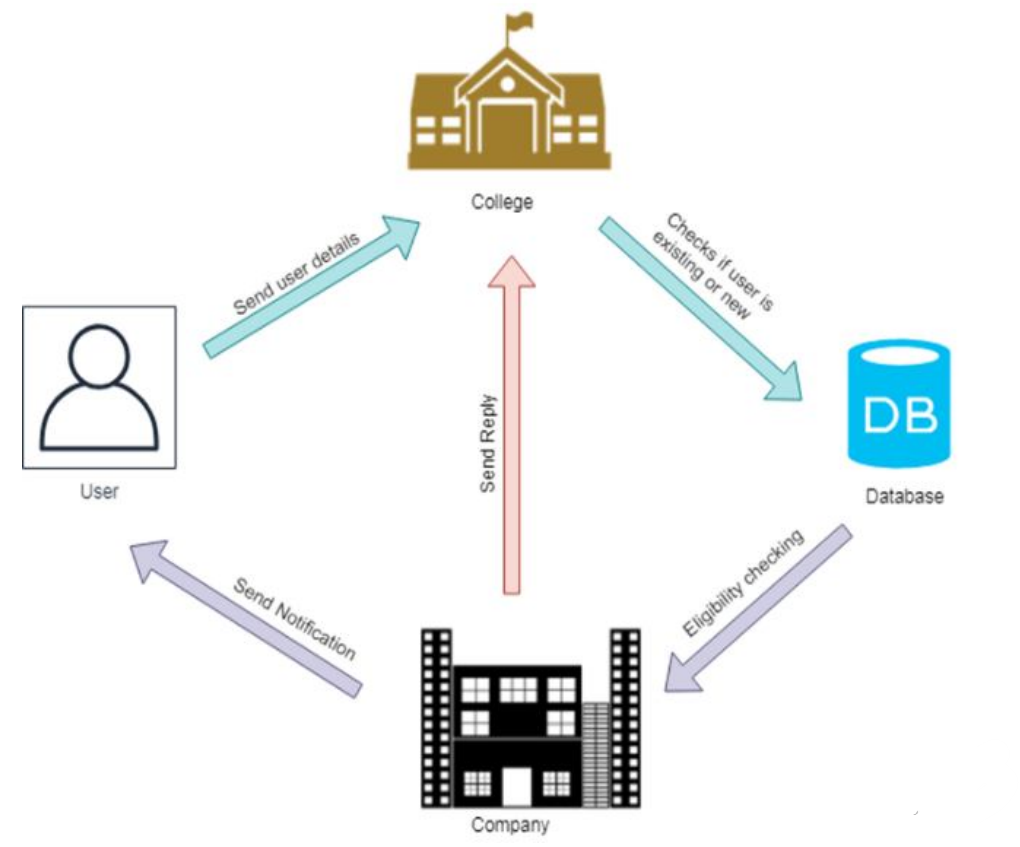
\includegraphics[width=10cm, height=10cm]{L1P1}
\caption{System Architecture}
\end{center}
\end{figure}

Ensemble methods is a machine learning 
technique that combines several base models in order to 
produce one optimal predictive model. To better understand 
this definition let’s take a step back into goal of machine 
learning and model building.

\begin{figure}[H]
\begin{center}
 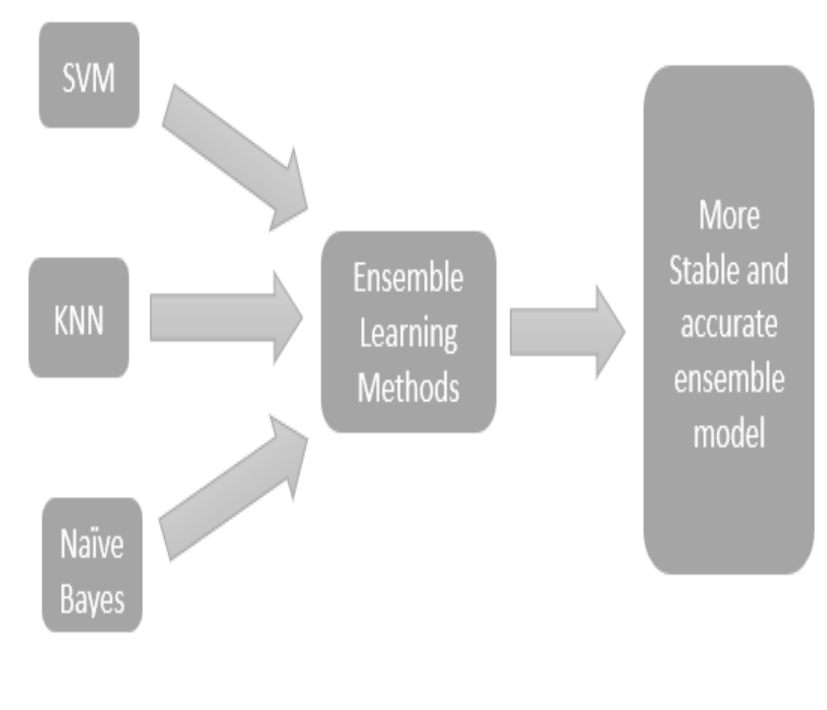
\includegraphics[width=10cm, height=3.9cm]{L1P2}
\caption{Ensemble Learning}
\end{center}
\end{figure}

The goal of any machine learning problem is to find a 
single model that will best predict our wanted outcome. Rather 
than making one model and hoping this model is the best/most 
accurate predictor I can make, ensemble methods take a 
myriad of models into account, and average those models to 
produce one final model.

This system is helpful for institutions to predict
student’s campus placement. This system would help reduce 
tedious job of manual placement system. The placement 
officer can work on identifying the weaknesses of each 
students and can suggest improvements so that the students 
can overcome the weakness and perform to the best of their 
abilities.

\newpage
\subsubsection{Advantages}
\begin{itemize}
\item Ensemble methods have higher predictive accuracy, compared to the individual models.
\item Ensemble of models is always less noisy and is more stable. 
\item It reduces the tedious job of manual placement system. 
\end{itemize}
\vspace{10px}
\par \subsubsection{Disadvantages}
\begin{itemize}
\item The art of ensembling is hard to learn and any wrong selection can lead to lower predictive accuracy than an individual model.
\item Ensembling is less interpretable, the output of the ensembled model is hard to predict and explain.
\item Ensembling is expensive in terms of both time and space.
\item It takes more time to compute.
\end{itemize}
\vspace{10px}
\newpage

\subsection{Use of ID3 Decision Tree Algorithm for Placement Prediction}
\vspace*{10px}

\subsubsection{Introduction}
Every year corporate companies come to 
colleges in order to recruit students. Recruitment is one of the 
most essential processes for any organization as they look for 
skilled and qualified professionals to fill up the positions in 
their organization. Many companies hire students through 
campus recruitment process. 

Campus recruitment is an 
efficient way to get the right resources at the right time with 
minimal cost and within minimum time frame. While the 
industry hires candidates from different institutes, students 
too get a chance to start their career with some of the best 
companies in the corporate sector.
The main aim of this paper is to identify relevant attributes based on quantitative and 
qualitative aspects of a student's profile such as CGPA, 
academic performance, technical and communication skills 
and design a model which can predict the placement of a 
student. 

For this purpose ID3 classification technique based 
on decision tree has been used. The result of this analysis will 
assist the academic planners to design a strategy to improve 
the performance of students that will help them in getting 
placed at the earliest.

\newpage
\subsubsection{Working}
Campus placement is a process where companies come 
to colleges and identify students who are talented and 
qualified, before they finish their graduation. The proposed 
system determines the likelihood of placement based on 
various attributes of a student’s profile. Depending on the 
parameters , manual classification is done whether the 
student is placed or not placed. A decision tree is then 
implemented to determine the probable outcome of a 
student being placed.

\begin{figure}[H]
\begin{center}
 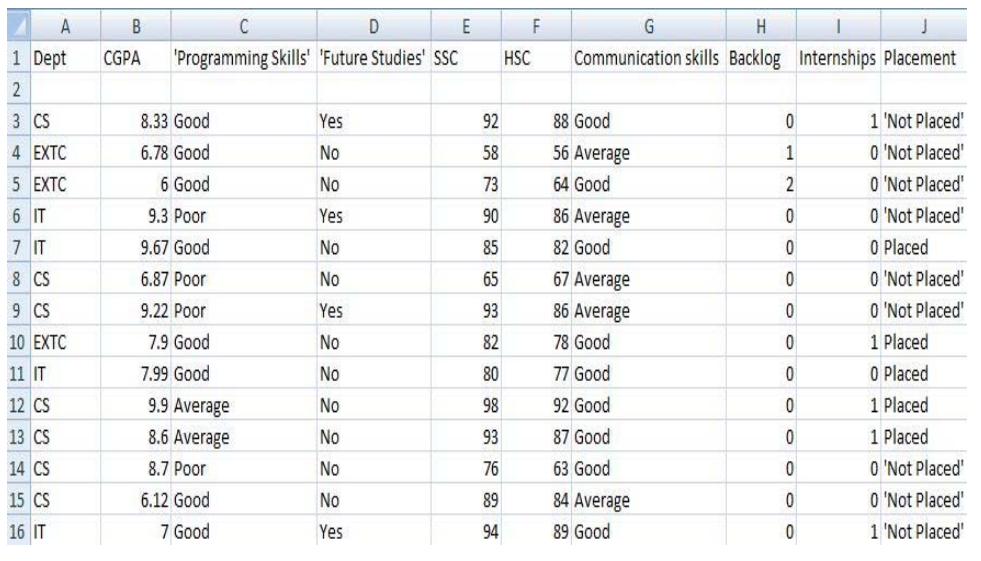
\includegraphics[width=10cm, height=8cm]{L2P2}
\caption{Student Data}
\end{center}
\end{figure}

The combination of various attributes determines 
whether the student is placed or not. The quantitative 
aspects like undergraduate CGPA, Marks obtained in X 
and XII form the major aspect of a student’s academic 
endeavours. The qualitative aspects like communication 
and programming skills form a backbone for a student to 
get placed as each recruiting company desires to hire 
students that have a sound technical knowledge and ability 
to communicate effectively. The other factors like 
internships, backlogs, future studies add value only when 
the prior requirements are met.

Based on the training set, information gain and entropy 
is calculated to determine the splitting attribute for 
constructing the decision tree. The algorithm gives a pruned decision tree with leaves as 
the decision that is placed or not placed. The primary node 
consists of programming skills which can accommodate 
three possible values viz. Good, Average and Poor. If the 
programming skills are Poor, the student is not placed. 
Furthermore, if the programming skills are good, the 
student may be placed based on the academic credential 
which is CGPA. If the CGPA of the student is above 7, 
student will be placed otherwise the student will not be 
placed. Also, if the student has average programming 
skills, he may still be placed based on other attributes like 
internships, future studies, communication skills, etc. 
 The final decision tree with four leaf nodes is obtained 
as shown below. The leaf nodes hold the value whether the 
student is placed or not placed.


\begin{figure}[H]
\begin{center}
 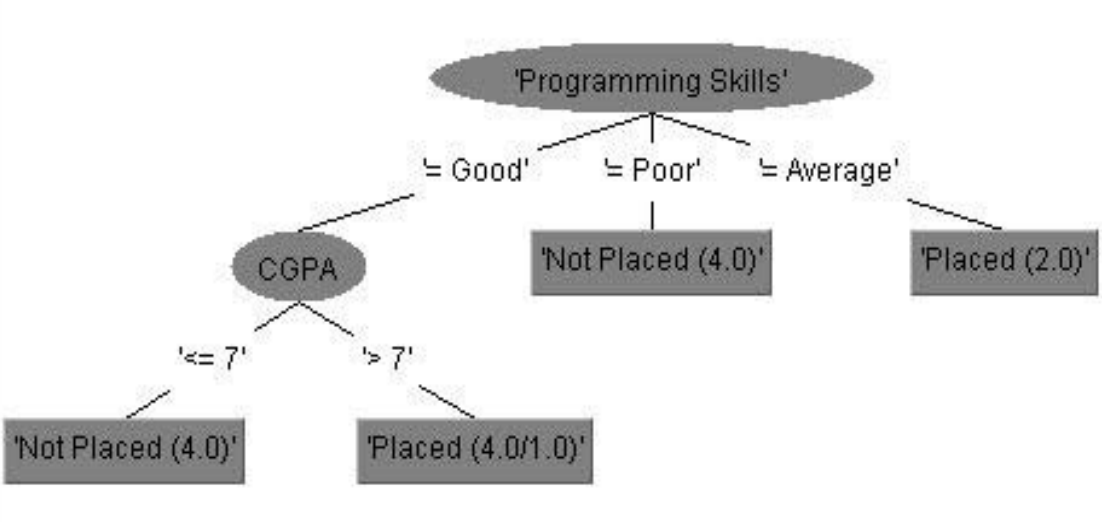
\includegraphics[width=10cm, height=6cm]{L2P1}
\caption{Decision Tree}
\end{center}
\end{figure}

The root node chosen here is Programming Skills. 
Further classification is done by calculating information 
gain and entropy for each attribute. Consider the attribute future studies; it has two possible 
classes viz. Yes and No. There are four students who wish 
to pursue future studies and remaining ten out of fourteen 
who do not have any plans to opt for higher studies. 
According to the training set, all the students who wish to 
pursue future studies are not placed. This indicates that all 
the information is contained in a single class. Hence, 
entropy becomes zero. Higher value of entropy indicates 
higher degree of distribution of information among classes. 
The lowest value of information gain is obtained for 
programming skills. Thus it is chosen as the root node. 
Further, the next lowest value (CGPA) is taken as the split 
node for next level. The subsequent nodes of decision tree 
at each level are determined by the value obtained in 
information gain.

In this paper ID3 classification algorithm is used to 
generate decision rule. The generated decision rule can be 
used to predict a student’s campus placement. The result of 
this algorithm can be used by the placement-in-charge to 
identify those set of students that are likely to face 
problems in campus placement. The classification model 
can play an important role in increasing the placement 
statistics. It can be concluded that classification algorithms 
can be used successfully in order to predict student 
placement. Further the implementation can be done in 
development and application of novel computational 
techniques for the analysis of large datasets.
\newpage
\subsubsection{Advantages}
\begin{itemize}
\item The best feature of using trees for analytics is that they are easy to interpret and explain. Decision trees are very intuitive and easy to explain.
\item  Nonlinear relationships between parameters do not affect tree performance.
\item Missing values in the data also do NOT affect the process of building a decision tree to any considerable extent. 
\item Compared to other algorithms decision trees requires less effort for data preparation during pre-processing.
\end{itemize}
\vspace{10px}
\subsubsection{Disadvantages}
\begin{itemize}
\item A small change in the data can cause a large change in the structure of the decision tree causing instability.
\item For a Decision tree sometimes calculation can go far more complex compared to other algorithms.
\item Decision tree often involves higher time to train the model.
\item Decision tree training is relatively expensive as the complexity and time has taken are more.
\end{itemize}
\newpage
\subsection{Student Prediction system for Placement training using Fuzzy inference System}
\vspace*{10px}
\subsubsection{Introduction}

Proposed student prediction system is most vital approach which may 
be used to differentiate the student data/information on the basis of the 
student performance. Managing placement and training records in 
any larger organization is quite difficult as the student number are 
high; in such condition differentiation and classification on different 
categories becomes tedious. 

Proposed fuzzy inference system will classify the student data with ease and will be helpful to many 
educational organizations. There are lots of classification algorithms 
and statistical base technique which may be taken as good assets for 
classify the student data set in the education field. 

In this paper, Fuzzy Inference system has been applied to predict student performance 
which will help to identify performance of the students and also 
provides an opportunity to improve to performance. For instance, here 
I will classify the student’s data set for placement and non-placement 
classes.
\newpage
\subsubsection{Working}

The main objective of this project is to classify large set of 
student data set using fuzzy logic and predicting student for 
placement training whether the student is eligible or not for 
placement training. As I discussed above I are taking two 
classes for final year student, classes are placement training and 
non-placement training. For the placement training those students 
will eligible those will get good marks or good CGPA in exam 
and remaining student will go for extra classes to improve their 
performance. From this approach I can predict all students in 
few times, if I want to classify all students on excel sheet so it 
will take lot of time, so these approaches are much better compare 
to other and it will help you. 

This proposal may also able to judge the performance of the 
student continuously. The main advantage of this system is to 
improve accuracy and speed of the student by conducting an exam 
and decide some criteria to pass that exam if student fails in exam 
than some important classes or training will provide to the student 
it will help to student to improve itself. The advantage of the 
system is the accuracy of the prediction and speed of the result 
provided. So the fuzzy system provides the easy way to classify 
several numbers of student data set. By making a fuzzy inference 
system and create some rules which will predict the student for 
pre-defined classes such as placement training and non-placement 
training.

\begin{figure}[H]
\begin{center}
 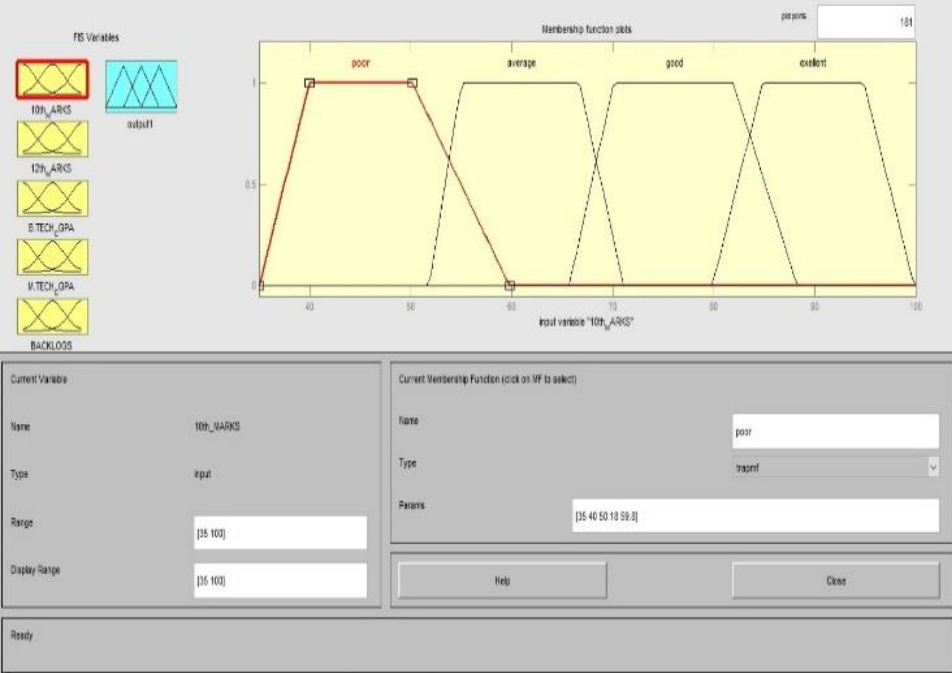
\includegraphics[width=10cm, height=6cm]{L3P1}
\caption{Fuzzy Inference System of each Input}
\end{center}
\end{figure}

For this system I collected 31 sample data set of M.Tech 
computer science student from our organization. In this data set 
put student registration number, name, 10th marks, 12th marks, 
B.Tech cgpa, M.Tech cgpa and number of backlogs. For 
classifying data set I skip some part of data set like registration 
number as well as name also here I take only academic marks 
and current backlog only and created more than 500 rules for 
predicting student performance for placement training on the 
basis of certain parameters. 

For example, if (10th marks is poor) 
and (12th marks is poor) and (B.Tech cgpa is poor) and (M.Tech 
cgpa is poor) and (backlog is less than 2) then (output is NO). 
From this fuzzy system can classify thousands number of 
student’s dataset. 
The main step of fuzzy based student prediction system is 
creating membership function for each input (10th marks, 12th
marks, B.Tech CGPA, M.Tech CGPA, and number of backlogs) 
and creates output in terms of eligibility corresponding inputs.

\begin{figure}[H]
\begin{center}
 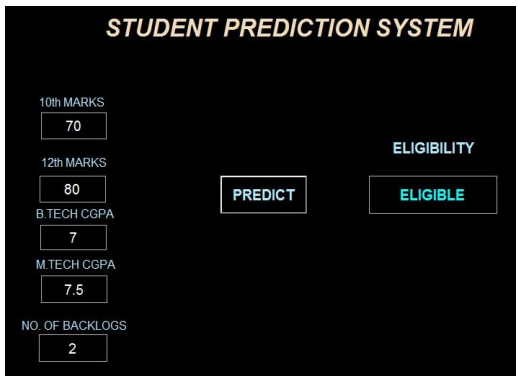
\includegraphics[width=10cm, height=6cm]{L3P2}
\caption{Output of Classified Individual student result}
\end{center}
\end{figure}

This system easily predicts and analyzes lot of student data set 
for predefined classes by using fuzzy logic which will definitely 
be a good asset to organization to analyze the information of huge 
number of student information and data sets. Future studies are 
required to investigate new hybrid models of fuzzy classification 
algorithms to improve the performance of prediction system.

\newpage
\subsubsection{Advantages}
\begin{itemize}
\item It is a robust system where no precise inputs are required.
\item The Fuzzy Logic algorithms can be coded using less data, so they do not occupy a huge memory space.
\item As it resembles human reasoning, these systems are able to solve complex problems where ambiguous inputs are available and take decisions accordingly.
\item These systems are flexible and the rules can be modified.
\end{itemize}
\vspace{10px}
\subsubsection{Disadvantages}
\begin{itemize}
\item There is no single systematic approach to solve a problem using Fuzzy Logic. As a result, many solutions arise for a particular problem, leading to confusion.
\item A major drawback of Fuzzy Logic control systems is that they are completely dependent on human knowledge and expertise.
\item You have to regularly update the rules of a Fuzzy Logic control system.
\end{itemize}


\newpage
\subsection{Student Placement Prediction Using Support Vector machine Algorithm}
\subsubsection{Introduction}
Campus placement plays a vital role in every educational institution in helping students to achieve their goals.
All students dream to obtain a job offer in their hands before they leave their college. In this paper, a predictive model is 
designed which can predict whether a student get placed or not. 

The main objective of this project is to analyze the student’s academics data, aptitude data and predict the placement possibilities of students to have an idea about where they stand and what to be done to obtain a good placement. Which also aids to increase the placement percentage of the institutions?.

The data has been collected by the institution for which prediction is going to be done and by applying 
suitable data pre-processing techniques. The model is built by both training and test set which gives accuracy in 
prediction. Here I use a single supervised machine learning algorithm named support vector machine algorithm. This 
algorithm independently predicts the results and I then compare the efficiency of the algorithm, which is based on the 
dataset. This model will help the placement cell to focus on the potential students and help them to improve their technical 
and other skills.
\newpage
\subsubsection{Working}
In this paper I use machine learning techniques to predict the placement status of students based on a dataset. The 
parameters in the dataset which are considered for the prediction are Quantitative scores, Logical Reasoning scores, 
Verbal scores, Programming scores, CGPA, internal marks, external marks, list of students placed in a company The 
placement prediction is done by machine learning Algorithm using SVM.

\begin{figure}[H]
\begin{center}
 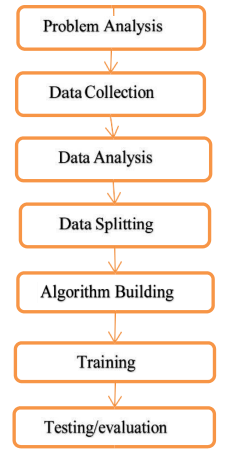
\includegraphics[width=10cm, height=10cm]{L4P1}
\caption{System Architecture}
\end{center}
\end{figure}

\begin{enumerate}
  \item  \textbf{Data Collection}
	     Sample data has been collected from college placement department. As an input for model prediction, which consist of all the required dataset.
  \item \textbf{Data Preparation \& Pre-processing}
	    Data preparation is a step in a data analysis process in which data from one or more sources is cleaned, transformed and enriched to improve the quality of data prior to its use. The collected data were then pre-processed to fill the missing data 
and made compatible for further processing.
  \item \textbf{Data Splitting}
Splitting the Dataset into Training set and Test Set ,Now the next step is to split our dataset into two. Training set and a 
Test set. I will train our machine learning models on our training set, i.e our machine learning models will try to 
understand any correlations in our training set and then I will test the models on our test set to examine how accurately 
it will predict. A general rule of the thumb is to assign 80% of the dataset to training set and therefore the remaining 20% 
to test set.
  \item \textbf{Algorithm Building}
SVM algorithm is appied on the dataset. SVM stands for Support Vector Machine. It is also a supervised machine learning 
algorithm that can be used for both classification and regression problems. However, it is mostly used for classification 
problems. A point in the n-dimensional space is a data item where the value of each feature is the value of a particular 
coordinate. Here, n is the number of features you have. After plotting the data item, I perform classification by finding 
the hyper-plane that differentiates the two classes very well. Now the problem lies in finding which hyper-plane to be 
chosen such that it is the right one. The Support Vector Machine (SVM) helps in identifying the hyperplane for 
classifying the data samples. In the case of multiple hyperplanes, the one which has maximum distance from the data 
points was chosen for better classification.
  \item \textbf{Evaluation and Testing:}
The performance measurement of the model was evaluated with the help of various metrics like accuracy, sensitivity, 
F1-score and precision. The performance visualization of the multi-class classification problem was analyzed using a 
graphical plot AUC (Area under the Curve) ROC (Receiver Operating Characteristics) curve that reveals the analytical 
ability of a binary classifier system as its discrimination threshold. The ROC curve is generated by plotting the true 
positive rate against false-positive rates at various threshold rates. The best algorithm based on the performance 
parameters was selected to predict the placement category of students. Based on the details provided by the students, the 
placement category could be predicted and the result would be displayed along with the suggestions for further 
improvement.
\end{enumerate}

From the study it is clear that the student dataset containing academic and placement details are a potential source for 
predicting the future placement chances and It is clear that SVM gives an accuracy of 100. This prediction can enlighten 
students to identify their capabilities and improve accordingly. This system also helps in the academic planning of an 
institution to prepare proper strategies and improve the placement statistics for the future years.

\newpage

\subsubsection{Advantages}
\begin{itemize}
\item SVM works relatively well when there is a clear margin of separation between classes.
\item SVM is more effective in high dimensional spaces \& SVM is relatively memory efficient.
\item SVM is effective in cases where the number of dimensions is greater than the number of samples.
\end{itemize}
\vspace{10px}
\subsubsection{Disadvantages}
\begin{itemize}
\item SVM algorithm is not suitable for large data sets.
\item SVM does not perform very well when the data set has more noise i.e. target classes are overlapping. 
\item In cases where the number of features for each data point exceeds the number of training data samples, the SVM will underperform.
\end{itemize}
\vspace{10px}

\newpage
\subsection{Recruitment System with Placement Prediction}
\subsubsection{Introduction}
The availability of information and the 
facility for the user to take action on the information 
collected have been revolutionized by the use of the 
Internet and the World Wide Web. The placement 
process can be managed using the internet which 
arises a need to develop a web-based placement 
management system specifically by the recruiters and 
the software engineers that can be used as a 
Recruitment system (Online TnP portal). 

This system can be used as an application for both candidates and 
recruiters. Advanced features for recruiters are 
available as they can shortlist candidates for further 
rounds according to their requirements on the basis 
of the probability obtained. The current recruitment 
system recruiters do not possess candidate 
information apart from his/her CV. 

This proposed system aims to analyze the candidate performance 
and recommend candidates fittest for the job using 
Random Forest Regressor algorithm that will help to 
maximize the placement probability of candidates 
easing the recruiter’s task. Random Forest builds 
multiple decision trees and merges them together to 
get a more accurate and stable prediction. This 
system will provide ease and efficiency in recruitment 
process.

\newpage
\subsubsection{Working}
The proposed system is a Web application meant 
to be used for recruitment process. It can be used 
by organizations as a tool for effective 
recruitment by analyzing the candidate’s fitness 
for the job. And colleges can use the system to get 
an idea about the probability of the student to be 
placed prior to the placement drive with the help 
of Placement prediction feature. This system 
recommends the candidates on the basis of their 
likelihood to get placed. It considers parameters 
like candidate’s SSC marks, HSC marks, CGPA, 
gender to predict the placement probability. 
Machine learning technique is used to implement 
Random Forest Regressor algorithm. The model 
is first trained on a dataset of any previous 
placement drives and then used to predict the 
probability of the candidate to get placed.
The system consists of two phases – 
\begin{enumerate}
\item Real-time placement prediction system (dynamic).
\item Probable candidate list generator(static).
\end{enumerate}
\textbf{Real-time placement prediction system (dynamic):}

\begin{figure}[H]
\begin{center}
 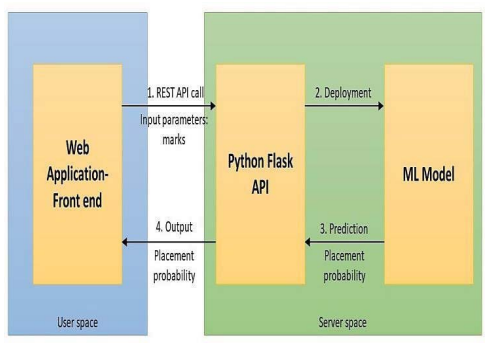
\includegraphics[width=10cm, height=6cm]{L5P1}
\caption{Dynamic predictor }
\end{center}
\end{figure}

This phase is for walk-in candidates where no 
previous record of him is available in the system. The following steps are carried out:

Step1: Placement candidate enters required credentials.
 
Step2: These input parameters will be passed to the Flask API using REST API call. 

Step3: The data forwarded by API will be given to trained ML model for calculation of placement probability. 

Step4: This placement probability will be displayed on the web page back through Flask API and the candidate record will be saved in a csv file. 

\textbf{ Probable candidate list generator(static):}

\begin{figure}[H]
\begin{center}
 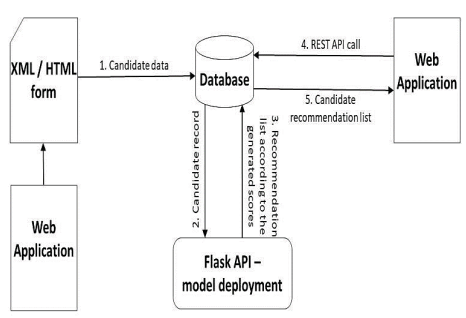
\includegraphics[width=10cm, height=6cm]{L5P2}
\caption{Static predictor }
\end{center}
\end{figure}

This phase is for candidates who enter their data 
through a form or whose records are already 
present in the database of the system. 

Step1: HTML/XML form is filled by candidate to store data in database using browser. 

Step2: Flask API is used to implement ML algorithms on database data. 

Step3: A trained ML model is implemented on the candidate records and scores are generated. 

Step4: A candidate recommendation list is generated based on the scores. 

Step5: Whenever a placement client requests the list, it will be retrieved from database and displayed on the web page. 

Prediction Process in both phases:
A pickle file is created, in which scikit-learn is 
imported which is a Machine Learning module. 
Using scikit-learn, Random Forest Regressor 
algorithm is trained on a dataset which contains 
historic data of placement drive. 
Now this pickle file is read by the Flask API file 
and the trained model is fitted on the current 
candidate records.

The proposed system consisting of dynamic 
prediction uses Machine learning to predict the 
placement probability of candidates dynamically 
using the parameters such as CGPA, HSC marks, 
SSC marks. It overcomes the limitations of current 
recruitment system which displays discrete values 
and gives an idea about placement to the candidates. 
The Scikit learn module provides us with a Random 
Forest Regressor algorithm which helps in 
generating probabilities with accuracy for large 
datasets and hence is comfortably suited for this 
purpose.

\newpage

\subsubsection{Advantages}
\begin{itemize}
\item It reduces overfitting in decision trees and helps to improve the accuracy.
\item It is flexible to both classification and regression problems.
\item Normalising of data is not required as it uses a rule-based approach.
\item It works well with both categorical and continuous values \& it automates missing values present in the data.
\end{itemize}
\vspace{10px}
\subsubsection{Disadvantages}
\begin{itemize}
\item It requires much computational power as well as resources as it builds numerous trees to combine their outputs.
\item It also requires much time for training as it combines a lot of decision trees to determine the class.
\item Due to the ensemble of decision trees, it also suffers interpretability and fails to determine the significance of each variable.
\end{itemize}
\vspace{10px}

\newpage

\begin{flushleft}\textbf{CHAPTER 3} \end{flushleft}
\begin{flushleft}\section{PROBLEM STATEMENT} \end{flushleft}
Previous Literatures Survey's have used machine learning algorithms like :
\begin{enumerate}
\item Ensemble learning (with SVM, KNN and Naive Bayes) for recruiters and colleges to predict the placement.
\item ID3 algorithm for academic planner to predict the placement.
\item Fuzzy logic for analyzing student perfomance to predict the placement.
\item SVM for placement cell to predict the placement.
\item Random forest regressor for recruiters to predict the placement.
\end{enumerate}
Eventhough the algorithms has classified the placement probablity as can be Placed or not, the expected accuracy was not attained with any of the above mentioned algorithm as the used data set was small, algorithm was complex, algorithm was not efficient etc... . 
So in this paper I have decided to use huge dataset and select the best algorithms out of the following:
\begin{enumerate}
\item Logistic Regression
\item KNN Algorithm
\item SVM Algorithm
\item XGBoost Classifier
\item Decision Tree Algorithm
\end{enumerate}
\newpage
\begin{flushleft}\textbf{CHAPTER 4} \end{flushleft}
\begin{flushleft}\section{PROPOSED SYSTEM} \end{flushleft}
\subsection{Introduction}
The importance of campus placement assistant system is to modify the present 
manual system where there the datas are in an unorganized manner. Due to unorganized data the stakeholders namely Placement Officers and Recruiters face difficulty in selecting the best student from the campus. The students should also need to have a clear picture of the placements going in the campus, so an effective computerized system will help the stakeholders to select the best student and the student to understand their level that is whether they can be placed or not.

The propsed system helps a student to get the placement details and can check for placement prediction, mock test and interview question this helps the student to have an environment where the student can get placement details. This also helps the admin or placement officer to get the details of student after prediction and the placemnt details from the company or recruiters can be directly passed to the students. 

\subsection{Technology used}
\subsubsection{Anvil}
Anvil is a new way to build web apps, with nothing but Python. This documentation will tell you all about how it works.
You do not need to know anything about HTML, Javascript or website development to use Anvil. All you need is some familiarity with the Python programming language.Anvil fills in these gaps by allowing you to build a full-stack web app using only Python. You can build a user interface with a simple drag and drop UI (or build it with code if you insist), plot with your favorite Python plotting library (Plotly, Matplotlib, etc.), and then deploy to the web in one click. No servers or containers to deal with.

\textbf{Structure of an Anvil app}

An Anvil app is made up of:
\begin{enumerate}
\item A User Interface, which you design with a drag-and-drop designer.
\item Client-side Python code, which runs in the web browser.
\item Server-side Python code, which runs on Anvil’s servers.
\item A built-in database (Data Tables), which stores your data.
\item Some Python code running on your computer, which can also interact with your app.
\end{enumerate}
What else you can do. Anvil also has built-in support for:
\begin{enumerate}
\item One-click hosting and deployment
\item Versioning your app with Git version control
\item Sending and receiving emails
\item Exposing and using HTTP APIs
\item Integrating with services from: Google, Microsoft, Facebook and anything else with a Python SDK!
\end{enumerate}

\textbf{Deep Notebook}

Deepnote is a seriously slick Python notebook, hosted in the cloud, with incredible real-time collaboration. It’s great for working with other data scientists. But what happens when you want to share your project with non-programmers? They need an easy-to-use interface – so you need to deploy what you’ve built. Deepnote has been used to integrate the machine learning code to Anvil.
\newpage
\subsubsection{Python Packages}
\textbf{NumPy}
NumPy is the fundamental package for scientific computing in Python. It is a Python library that provides a multidimensional array object, various derived objects (such as masked arrays and matrices), and an assortment of routines for fast operations on arrays, including mathematical, logical, shape manipulation, sorting, selecting, I/O, discrete Fourier transforms, basic linear algebra, basic statistical operations, random simulation and much more.

At the core of the NumPy package, is the ndarray object. This encapsulates n-dimensional arrays of homogeneous data types, with many operations being performed in compiled code for performance. There are several important differences between NumPy arrays and the standard Python sequences:
\begin{itemize}
\item NumPy arrays have a fixed size at creation, unlike Python lists (which can grow dynamically). Changing the size of an ndarray will create a new array and delete the original.
\item The elements in a NumPy array are all required to be of the same data type, and thus will be the same size in memory. The exception: one can have arrays of (Python, including NumPy) objects, thereby allowing for arrays of different sized elements.
\item NumPy arrays facilitate advanced mathematical and other types of operations on large numbers of data. Typically, such operations are executed more efficiently and with less code than is possible using Python’s built-in sequences.
\end{itemize}
\textbf{pandas}
\\
pandas is a Python package that provides fast, flexible, and expressive data structures designed to make working with "relational" or "labeled" data both easy and intuitive. It aims to be the fundamental high-level building block for doing practical, real world data analysis in Python. Additionally, it has the broader goal of becoming the most powerful and flexible open source data analysis / manipulation tool available in any language. It is already well on its way towards this goal.
Pandas makes it simple to do many of the time consuming, repetitive tasks associated with working with data, including:
\begin{itemize}
\item Data cleansing
\item Data fill
\item Data normalization
\item Merges and joins
\item Data visualization
\item Statistical analysis
\item Data inspection
\item Loading and saving data etc..
\end{itemize}

\textbf{Matplotlib}

Matplotlib is an amazing visualization library in Python for 2D plots of arrays. Matplotlib is a multi-platform data visualization library built on NumPy arrays and designed to work with the broader SciPy stack. It was introduced by John Hunter in the year 2002.One of the greatest benefits of visualization is that it allows us visual access to huge amounts of data in easily digestible visuals. Matplotlib consists of several plots like line, bar, scatter, histogram etc.
\textbf{Seaborn}
\\
Seaborn is a data visualization library built on top of matplotlib and closely integrated with pandas data structures in Python. Visualization is the central part of Seaborn which helps in exploration and understanding of data. One has to be familiar with Numpy and Matplotlib and Pandas to learn about Seaborn.

Seaborn offers the following functionalities:
\begin{itemize}
\item Dataset oriented API to determine the relationship between variables.
\item Automatic estimation and plotting of linear regression plots.
\item It supports high-level abstractions for multi-plot grids.
\item Visualizing univariate and bivariate distribution.
\end{itemize}

\newpage
\subsubsection{GitHub}
GitHub is a Git repository hosting service that provides a web-based graphical interface (GUI). It helps every team member work together on a project from anywhere, making it easy to collaborate. 

GitHub is one place where project managers and developers coordinate, track, and update their work, so projects stay transparent and on schedule. The packages can be published privately, within the team, or publicly for the open-source community. Downloading packages from GitHub enables them to be used and reused. GitHub helps all team members stay on the same page and stay organized. Moderation tools, like issue and pull request locking, helps the team focus on the code.

\textbf{GitHub Desktop}
GitHub Desktop is an application that enables GUI-based interaction with GitHub. Git provides a wide range of commands for Git activities like creating repositories, commits, pull requests, and so on. However, GitHub desktop provides GUI-based those activities using best practices with Git and GitHub. I can use GitHub desktop to do most of the Git commands with UI and clicks which makes collaboration and working with Git more flexible. You can connect to your account, create git repositories, add projects, do the changes, and commit easily with the interface. I will be doing hands-on with the GitHub desk in this article.

\subsubsection{XGBoost}
XgBoost stands for Extreme Gradient Boosting, which was proposed by the researchers at the University of Washington. It is a library written in C++ which optimizes the training for Gradient Boosting.

Before understanding the XGBoost, I first need to understand the trees especially the decision tree:
\textbf{Decision Tree:}
A Decision tree is a flowchart-like tree structure, where each internal node denotes a test on an attribute, each branch represents an outcome of the test, and each leaf node (terminal node) holds a class label. 

A tree can be “learned” by splitting the source set into subsets based on an attribute value test. This process is repeated on each derived subset in a recursive manner called recursive partitioning. The recursion is completed when the subset at a node all has the same value of the target variable, or when splitting no longer adds value to the predictions.

\textbf{Bagging:}
A Bagging classifier is an ensemble meta-estimator that fits base classifiers each on random subsets of the original dataset and then aggregate their individual predictions (either by voting or by averaging) to form a final prediction. Such a meta-estimator can typically be used as a way to reduce the variance of a black-box estimator (e.g., a decision tree), by introducing randomization into its construction procedure and then making an ensemble out of it.
Each base classifier is trained in parallel with a training set which is generated by randomly drawing, with replacement, N examples(or data) from the original training dataset, where N is the size of the original training set. The training set for each of the base classifiers is independent of each other. Many of the original data may be repeated in the resulting training set while others may be left out.

Bagging reduces overfitting (variance) by averaging or voting, however, this leads to an increase in bias, which is compensated by the reduction in variance though.

\begin{figure}[H]
\begin{center}
 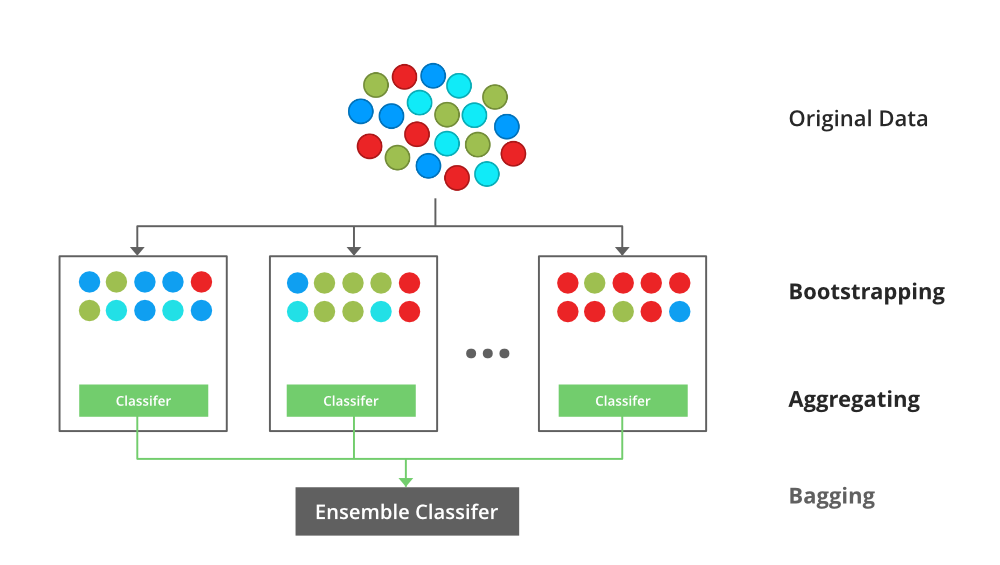
\includegraphics[width=10cm, height=6cm]{Tech1}
\caption{Bagging Classifier}
\end{center}
\end{figure}

\textbf{Random Forest:}
Every decision tree has high variance, but when I combine all of them together in parallel then the resultant variance is low as each decision tree gets perfectly trained on that particular sample data and hence the output doesn’t depend on one decision tree but multiple decision trees. In the case of a classification problem, the final output is taken by using the majority voting classifier. In the case of a regression problem, the final output is the mean of all the outputs. This part is Aggregation.
 

The basic idea behind this is to combine multiple decision trees in determining the final output rather than relying on individual decision trees.
Random Forest has multiple decision trees as base learning models. I randomly perform row sampling and feature sampling from the dataset forming sample datasets for every model. This part is called Bootstrap.

\textbf{Boosting:}
Boosting is an ensemble modelling, technique that attempts to build a strong classifier from the number of weak classifiers. It is done by building a model by using weak models in series. Firstly, a model is built from the training data. Then the second model is built which tries to correct the errors present in the first model. This procedure is continued and models are added until either the complete training data set is predicted correctly or the maximum number of models are added.

\begin{figure}[H]
\begin{center}
 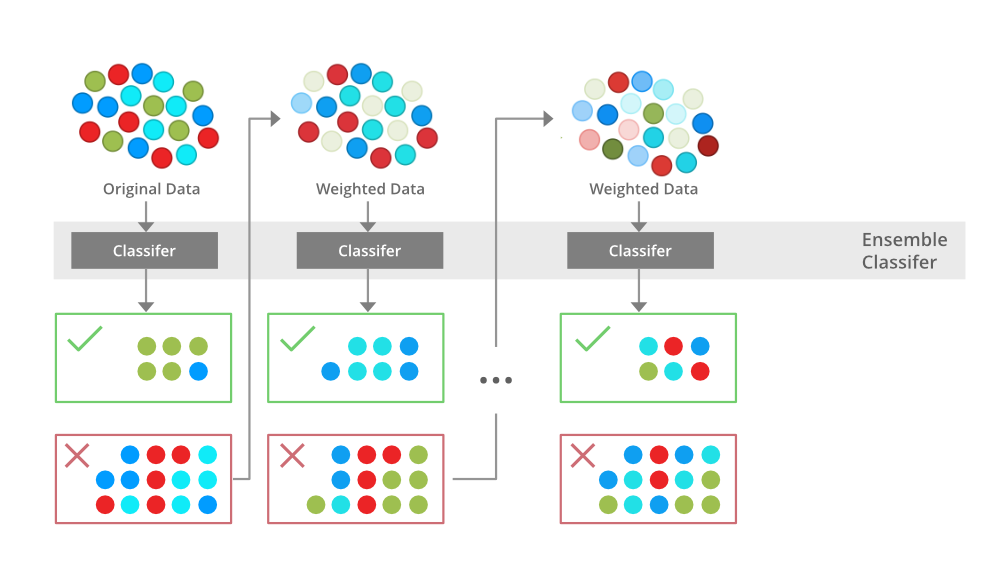
\includegraphics[width=10cm, height=6cm]{Tech2}
\caption{Boosting}
\end{center}
\end{figure}

\textbf{Gradient Boosting }
Gradient Boosting is a popular boosting algorithm. In gradient boosting, each predictor corrects its predecessor’s error. In contrast to Adaboost, the weights of the training instances are not tweaked, instead, each predictor is trained using the residual errors of predecessor as labels.

There is a technique called the Gradient Boosted Trees whose base learner is CART (Classification and Regression Trees).

\textbf{XGBoost }
XGBoost is an implementation of Gradient Boosted decision trees. XGBoost models majorly dominate in many Kaggle Competitions.In this algorithm, decision trees are created in sequential form. Weights play an important role in XGBoost. Weights are assigned to all the independent variables which are then fed into the decision tree which predicts results. The weight of variables predicted wrong by the tree is increased and these variables are then fed to the second decision tree. These individual classifiers/predictors then ensemble to give a strong and more precise model. It can work on regression, classification, ranking, and user-defined prediction problems.

\textbf{Features of XGBoost}
\begin{enumerate}
\item\textbf{Regularization:} Since the ensembling of decisions, trees can sometimes lead to very complex. XGBoost uses both Lasso and Ridge Regression regularization to penalize the highly complex model.
\item\textbf{Parallelization} and Cache block: In, XGboost, I cannot train multiple trees parallel, but it can generate the different nodes of tree parallel. For that, data needs to be sorted in order. In order to reduce the cost of sorting, it stores the data in blocks. It stored the data in the compressed column format, with each column sorted by the corresponding feature value. This switch improves algorithmic performance by offsetting any parallelization overheads in computation.
\item\textbf{Tree Pruning:}  XGBoost uses max\_depth parameter as specified the stopping criteria for the splitting of the branch, and starts pruning trees backward. This depth-first approach improves computational performance significantly.
\item\textbf{Cache-Awareness and Out-of-score computation:} This algorithm has been designed to make use of hardware resources efficiently. This is accomplished by cache awareness by allocating internal buffers in each thread to store gradient statistics. Further enhancements such as ‘out-of-core computing optimize available disk space while handling big data-frames that do not fit into memory. In out-of-core computation, Xgboost tries to minimize the dataset by compressing it.
\item\textbf{Sparsity Awareness:} XGBoost can handle sparse data that may be generated from preprocessing steps or missing values. It uses a special split finding algorithm that is incorporated into it that can handle different types of sparsity patterns.
\item\textbf{Weighted Quantile Sketch:} XGBoost has in-built the distributed weighted quantile sketch algorithm that makes it easier to effectively find the optimal split points among weighted datasets.
\item\textbf{Cross-validation:} XGboost implementation comes with a built-in cross-validation method. This helps the algorithm prevents overfitting when the dataset is not that big.
\end{enumerate}

\newpage
\begin{flushleft}\textbf{CHAPTER 5} \end{flushleft}
\begin{flushleft}\section{FEASIBILITY STUDY} \end{flushleft}
\vspace*{10px}
All projects are feasible when given unlimited resources and infinite time. It is both
necessary and prudent to evaluate the feasibility of a project at the earliest possible
time. An estimate is made of whether the identified user needs may be satisfied using
current software and hardware technologies. The study will decide if the proposed
system will be cost effective from the business point of view and if it can be developed
in the given existing budgetary constraints. The feasibility study should be relatively
cheap and quick. The result should inform the decision of whether to go ahead with a
more detailed analysis. Feasibility analysis is the procedure for identifying the candidate
system, evaluating and electing the most feasible system. This is done by investigating
the existing system in the area under investigation or generally ideas about a new
system. It is a test of a system proposal according to its work ability, impact on the
organization, ability to meet user needs, and effective use of resources. The objective
of feasibility study is not to solve the problem but to acquire a sense of its scope.
Feasibility analysis involves following steps
\begin{itemize}
\item  Form a project and appoint a project leader
\item Prepare system flowcharts
\item Create a web site
\item Weigh system performance and cost data
\item Prepare and report final project directive to management The study is done in
these phases
\item Operational feasibility
\item Technical feasibility
\item Economical feasibility
\item Behavioral feasibility
\item Software feasibility
\item Hardware feasibility
\end{itemize}
\subsection{ Operational Feasibility}
Proposed projects are beneficial only if they can be turned into information system
that will meet the organization’s operating requirements. Simply stated, this test of
feasibility asks if the system will work when it is developed and installed. Are there
major barriers to implementation? Here are questions that will help test the operational
feasibility of a project:
Is there sufficient support for the projects from management?
Are current business methods acceptable to the users?
Have the users been involved in the planning and development of the project?
Will the proposed system cause harm? The purpose of the operational feasibility
study is to determine whether the new system will be used if it is developed and
implemented. And whether there will be resistance from users that will undermine the
possible application benefits
\subsection{Technical Feasibility}
A study of function performance and constraints may improve the ability to create an
acceptable system. Technical feasibility is frequently the most difficult area to achieve
at the stage of product engineering process. Considering that are normally associated
with the technical feasibility include
\begin{itemize}
\item Development risk
\item Resource availability
\item Technology Technical feasibility study deals with the hardware as well as software
requirements. The scope was whether the work for the project is done with the current
equipments and the existing software technology has to be examined in the feasibility
study. The outcome was found to be positive. In proposed system, data can be easily
stored and managed using database management system software. The reports and
results for queries can be generated easily. Thus, system is technically feasible.

\end{itemize}


\subsection{Economical Feasibility  }

A cost evaluation is weighed against the ultimate income or benefit derived from
the developed system or product. When compared to the advantage obtained from
implementing the system its cost is affordable. Also the system is designed to meet the
modifications required in the future. So, most of the required modifications can be done
without much re-work. Proposed system was developed with the available resources.
Since cost input for the software is almost nil the output of the software is always a
profit. Hence software is economically feasible. In the existing system, manpower is
required. In the proposed system, number of employee



\subsection{Behavioral Feasibility }
People are inherently resistant to changes and computer is known for facilitating the
changes. An estimate should be made of how strongly the user staff reacts towards the
developments of the computerized system. In the existing system more manpower is
required and time factor is more. In proposed system, both man power and time factors
are reduced and also unnecessary burden is reduced. Thus the remaining people are
made to engage in some other important work. Therefore, the system is behaviorally
feasible.
\subsection{ Software Feasibility}

Even though software is developed in a very high software environment, it will be
sup- ported by many other platform and environments with minimum changes.

\subsection{ Hardware Feasibility}

The software can be developed with resource already existing. Here the consideration
is that the existing hardware resources support the technologies that are to be used by
the new system. No hardware was newly bought for the project and hence. Software
is to achieve hardware feasibility.

\newpage
\begin{flushleft}\textbf{CHAPTER 6} \end{flushleft}
\begin{flushleft}\section{REQUIREMENT SPECIFICATION} \end{flushleft}
\vspace*{10px}

\subsection{Software Requirements}
\begin{itemize}
\item Python (Version 3.0+)
\item Anvil
\item GitHub
\item DeepNote
\item ipynb file
\end{itemize}

\subsubsection{User Requirements}
\begin{itemize}
\item Any Web Browser
\end{itemize}

\subsection{Hardware Requirements}
\subsubsection{Development Requirements}
\begin{itemize}
\item Intel 7th gen i3 / AMD Ryzen 3
\item 4GB RAM
\item Hard Disk 8GB or more
\end{itemize}

\subsubsection{User Requirements}
\begin{itemize}
\item Intel Pentium / AMD A6
\item 512 MB RAM
\item 112 GB Storage space
\end{itemize}

\newpage
\begin{flushleft}\textbf{CHAPTER 7} \end{flushleft}
\begin{flushleft}\section{SYSTEM DESIGN} \end{flushleft}
\vspace*{10px}

\subsection{Data Flow Diagram}

DFD is the abbreviation for Data Flow Diagram. The flow of data of a system or a process is represented by DFD. It also gives insight into the inputs and outputs of each entity and the process itself. DFD does not have control flow and no loops or decision rules are present. Specific operations depending on the type of data can be explained by a flowchart. Data Flow Diagram can be represented in several ways. The DFD belongs to structured-analysis modeling tools. Data Flow diagrams are very popular because they help us to visualize the major steps and data involved in software-system processes.

In Software engineering DFD(data flow diagram) can be drawn to represent the system of different levels of abstraction. Higher-level DFDs are partitioned into low levels-hacking more information and functional elements. Levels in DFD are numbered 0, 1, 2 or beyond. Here, I will see mainly 3 levels in the data flow diagram, which are: 0-level DFD, 1-level DFD, and 2-level DFD. 	

\begin{itemize}

\item \textbf{0-level DFD: }
It is also known as a context diagram. It’s designed to be an abstraction view, showing the system as a single process with its relationship to external entities. It represents the entire system as a single bubble with input and output data indicated by incoming/outgoing arrows. 

\begin{figure}[H]
\begin{center}
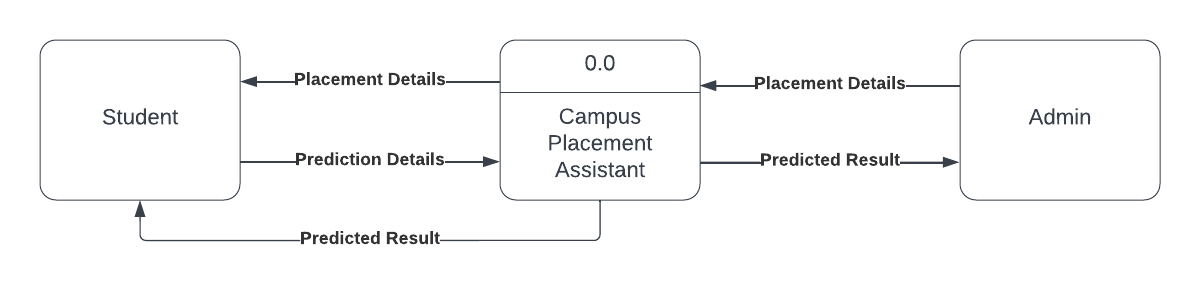
\includegraphics[scale=0.8]{0-LEVEL DFD}
\caption{0-level DFD}
\end{center}
\end{figure}

\item \textbf{1-level DFD: }
In 1-level DFD, the context diagram is decomposed into multiple bubbles/processes. In this level, I highlight the main functions of the system and breakdown the high-level process of 0-level DFD into subprocesses. 

\begin{figure}[H]
\begin{center}
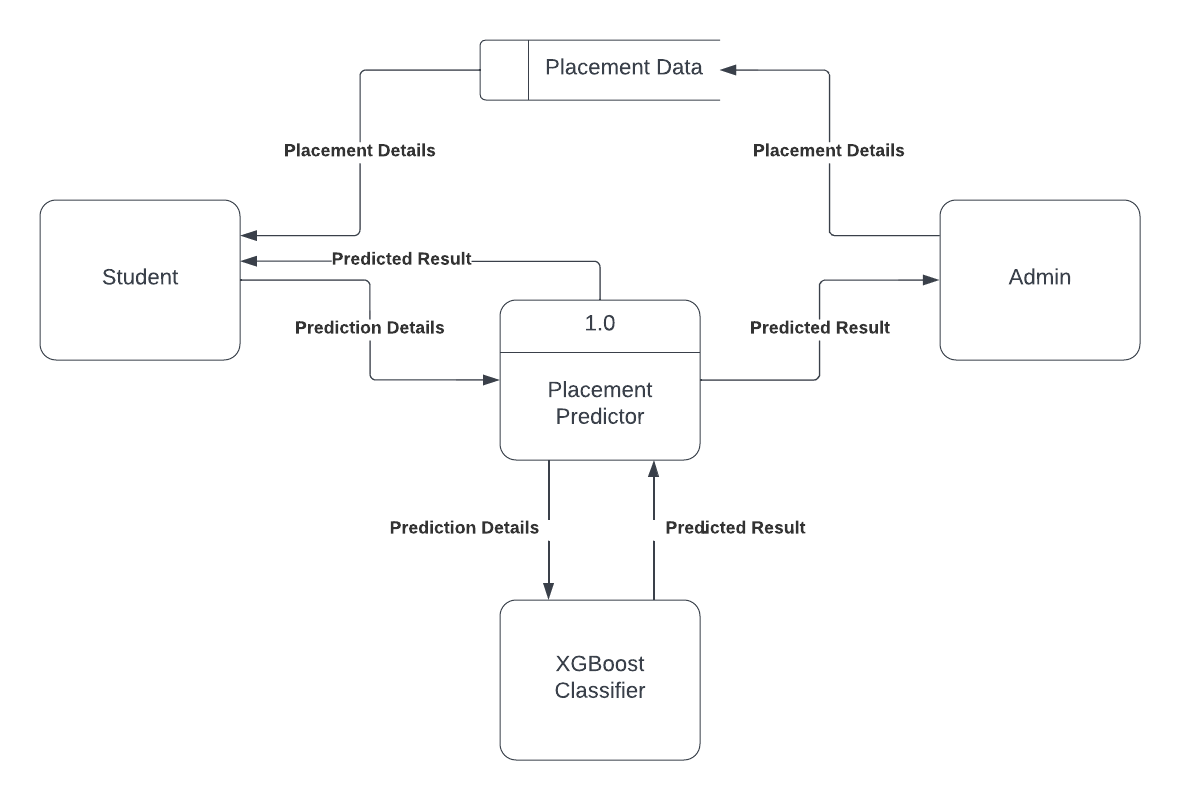
\includegraphics[scale=.8]{1-LEVEL DFD}
\caption{1-level DFD}
\end{center}
\end{figure}

\item \textbf{2-level DFD: }
2-level DFD goes one step deeper into parts of 1-level DFD. It can be used to plan or record the specific/necessary detail about the system’s functioning. 

\begin{figure}[H]
\begin{center}
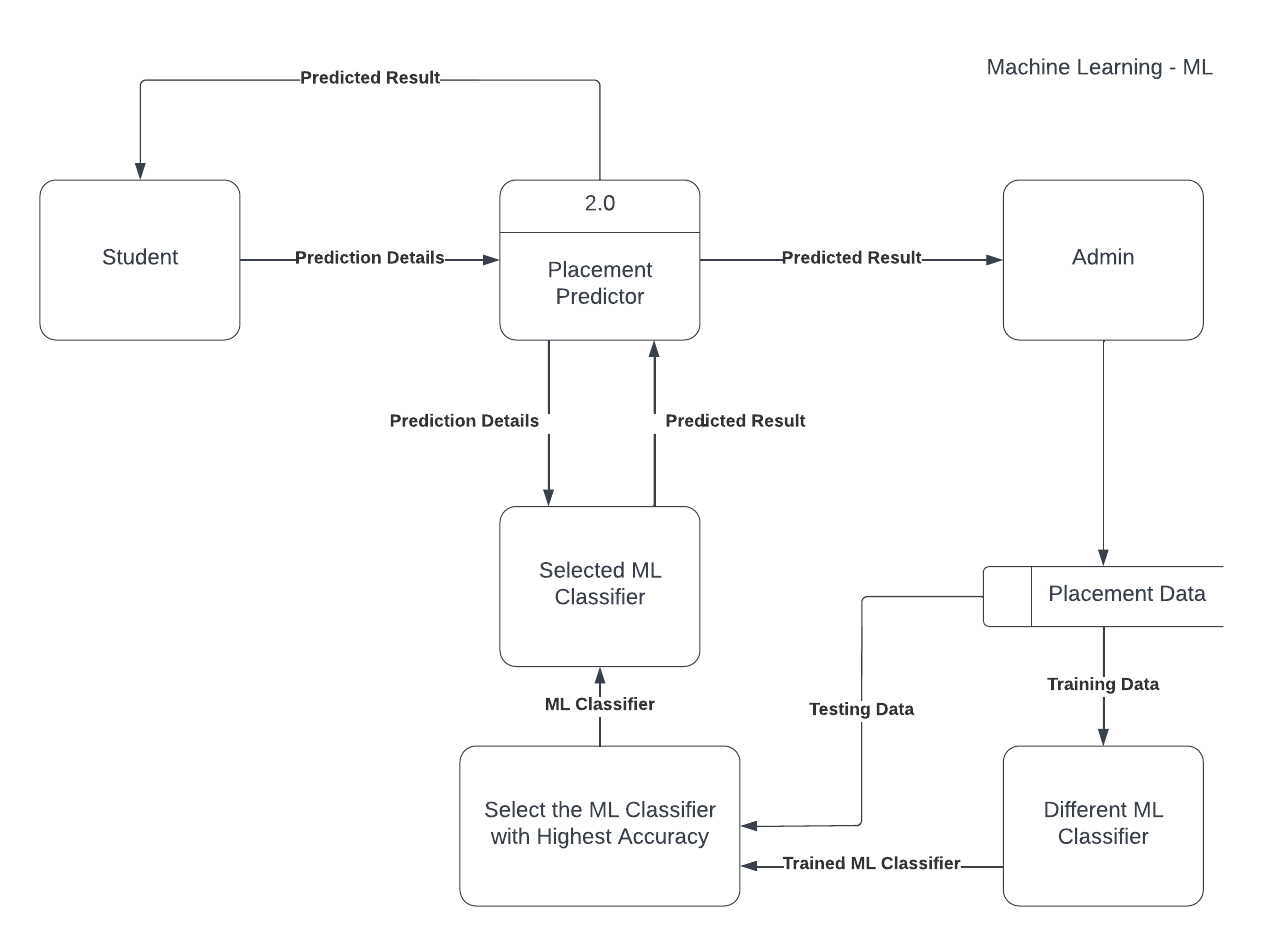
\includegraphics[scale=.8]{2- LEVEL DFD}
\caption{2-level DFD}
\end{center}
\end{figure}

\end{itemize}

\subsection{UML DIAGRAMS}

It is the general-purpose modeling language used to visualize the system. It is a graphical language that is standard to the software industry for specifying, visualizing, constructing, and documenting the artifacts of the software systems, as well as for business modeling.
Benefits of UML: 
\begin{itemize}
\item Simplifies complex software design, can also implement OOPs like a concept that is widely used.
\item It reduces thousands of words of explanation in a few graphical diagrams that may reduce time consumption to understand.
\item It makes communication more clear and more real.
\item It helps to acquire the entire system in a view.
\item It becomes very much easy for the software programmer to implement the actual demand once they have a clear picture of the problem.
\end{itemize}

\subsubsection{Sequence Diagram}

The sequence diagram represents the flow of messages in the system and is also termed as an event diagram. It helps in envisioning several dynamic scenarios. It portrays the communication between any two lifelines as a time-ordered sequence of events, such that these lifelines took part at the run time. In UML, the lifeline is represented by a vertical bar, whereas the message flow is represented by a vertical dotted line that extends across the bottom of the page. It incorporates the iterations as well as branching.

\begin{figure}[H]
\begin{center}
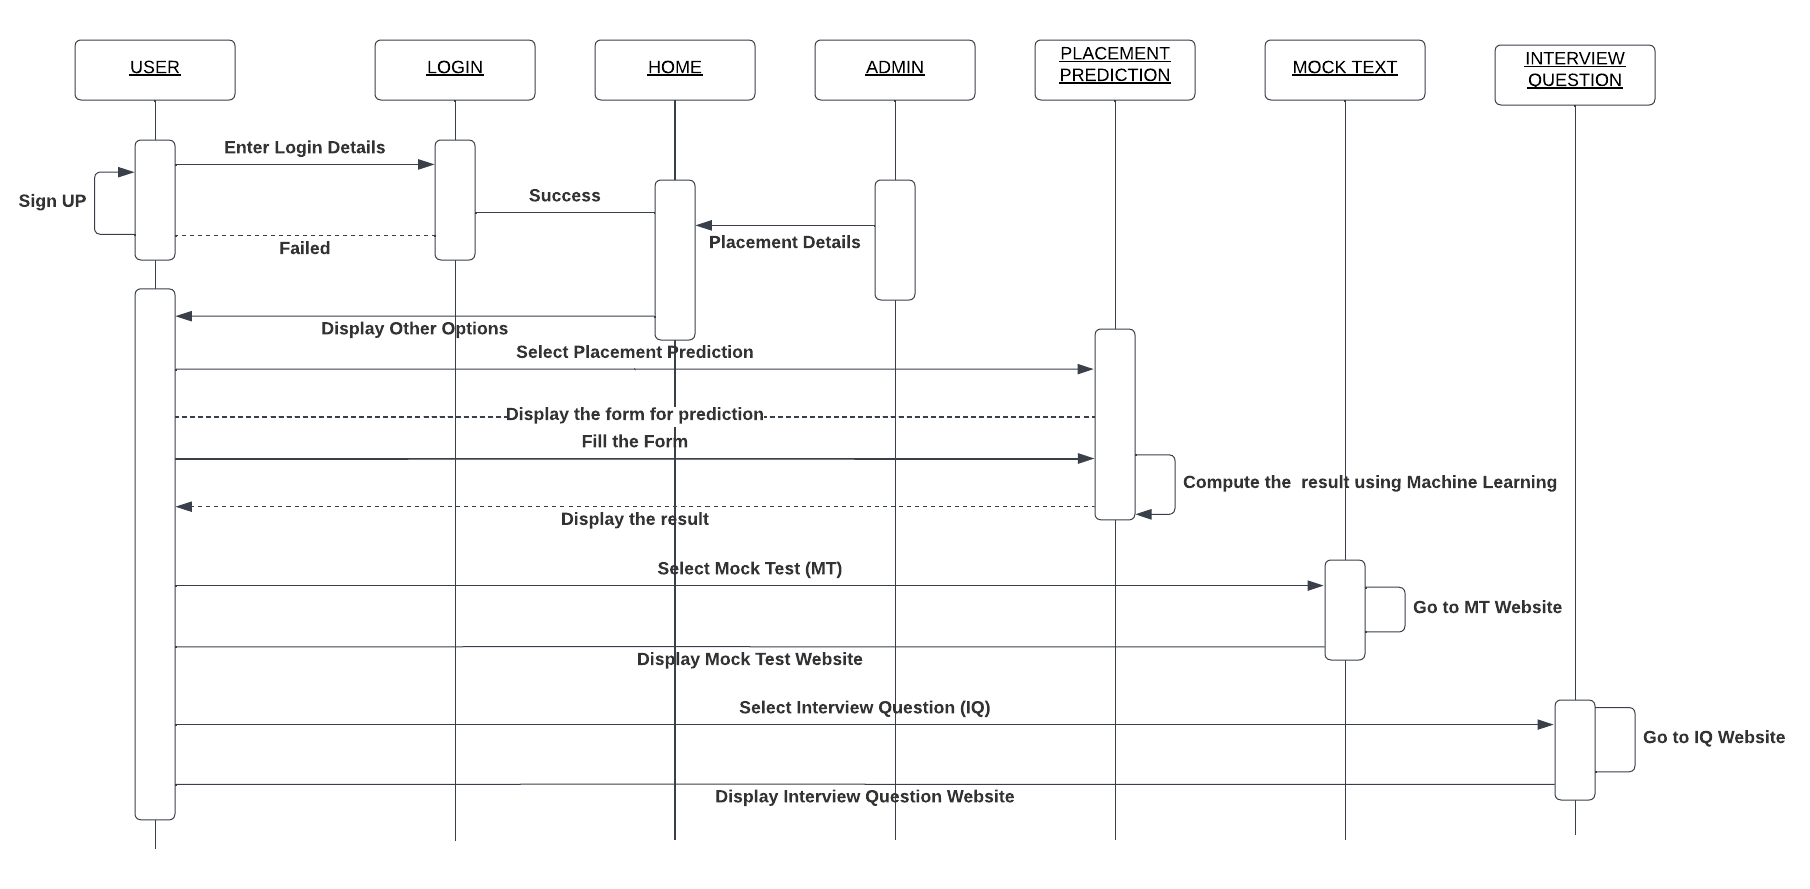
\includegraphics[scale=.6]{Sequence diagram}
\caption{Sequence Diagram}
\end{center}
\end{figure}

\subsubsection{Use Case Diagram}

A use case diagram is used to represent the dynamic behavior of a system. It encapsulates the system's functionality by incorporating use cases, actors, and their relationships. It models the tasks, services, and functions required by a system/subsystem of an application. It depicts the high-level functionality of a system and also tells how the user handles a system.

\begin{figure}[H]
\begin{center}
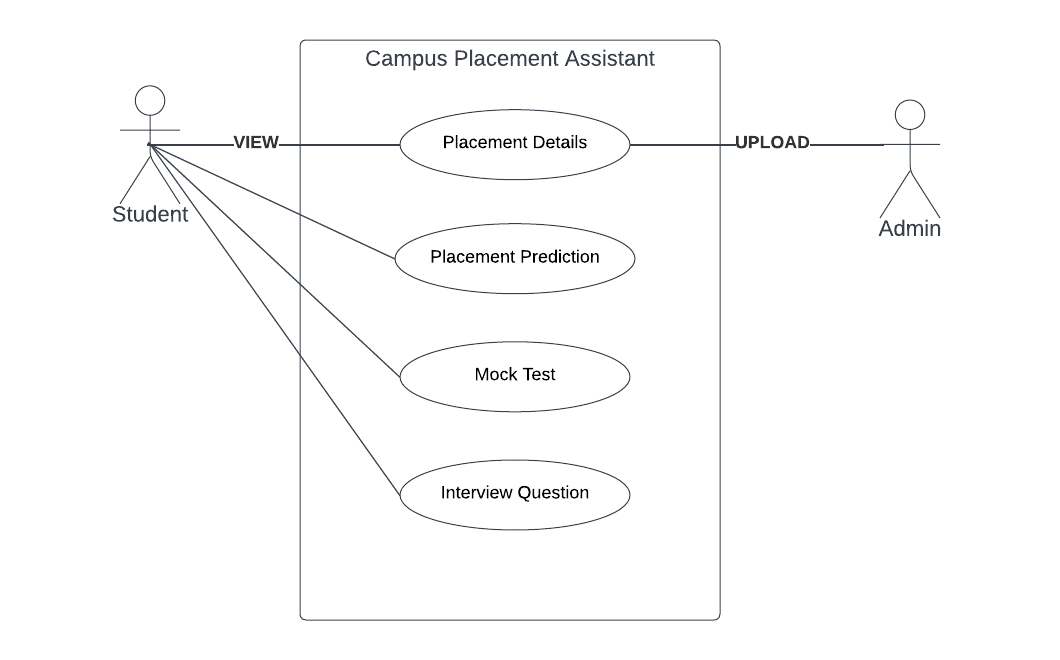
\includegraphics[scale=.8]{use case diagram}
\caption{Use Case Diagram}
\end{center}
\end{figure}

\newpage
\subsubsection{Activiy Diagram}

An activity diagram is a behavioral diagram i.e. it depicts the behavior of a system. An activity diagram portrays the control flow from a start point to a finish point showing the various decision paths that exist while the activity is being executed. I can depict both sequential processing and concurrent processing of activities using an activity diagram. They are used in business and process modelling where their primary use is to depict the dynamic aspects of a system. An activity diagram is very similar to a flowchart.

\vspace*{10px}
\begin{figure}[h!]
\begin{center}
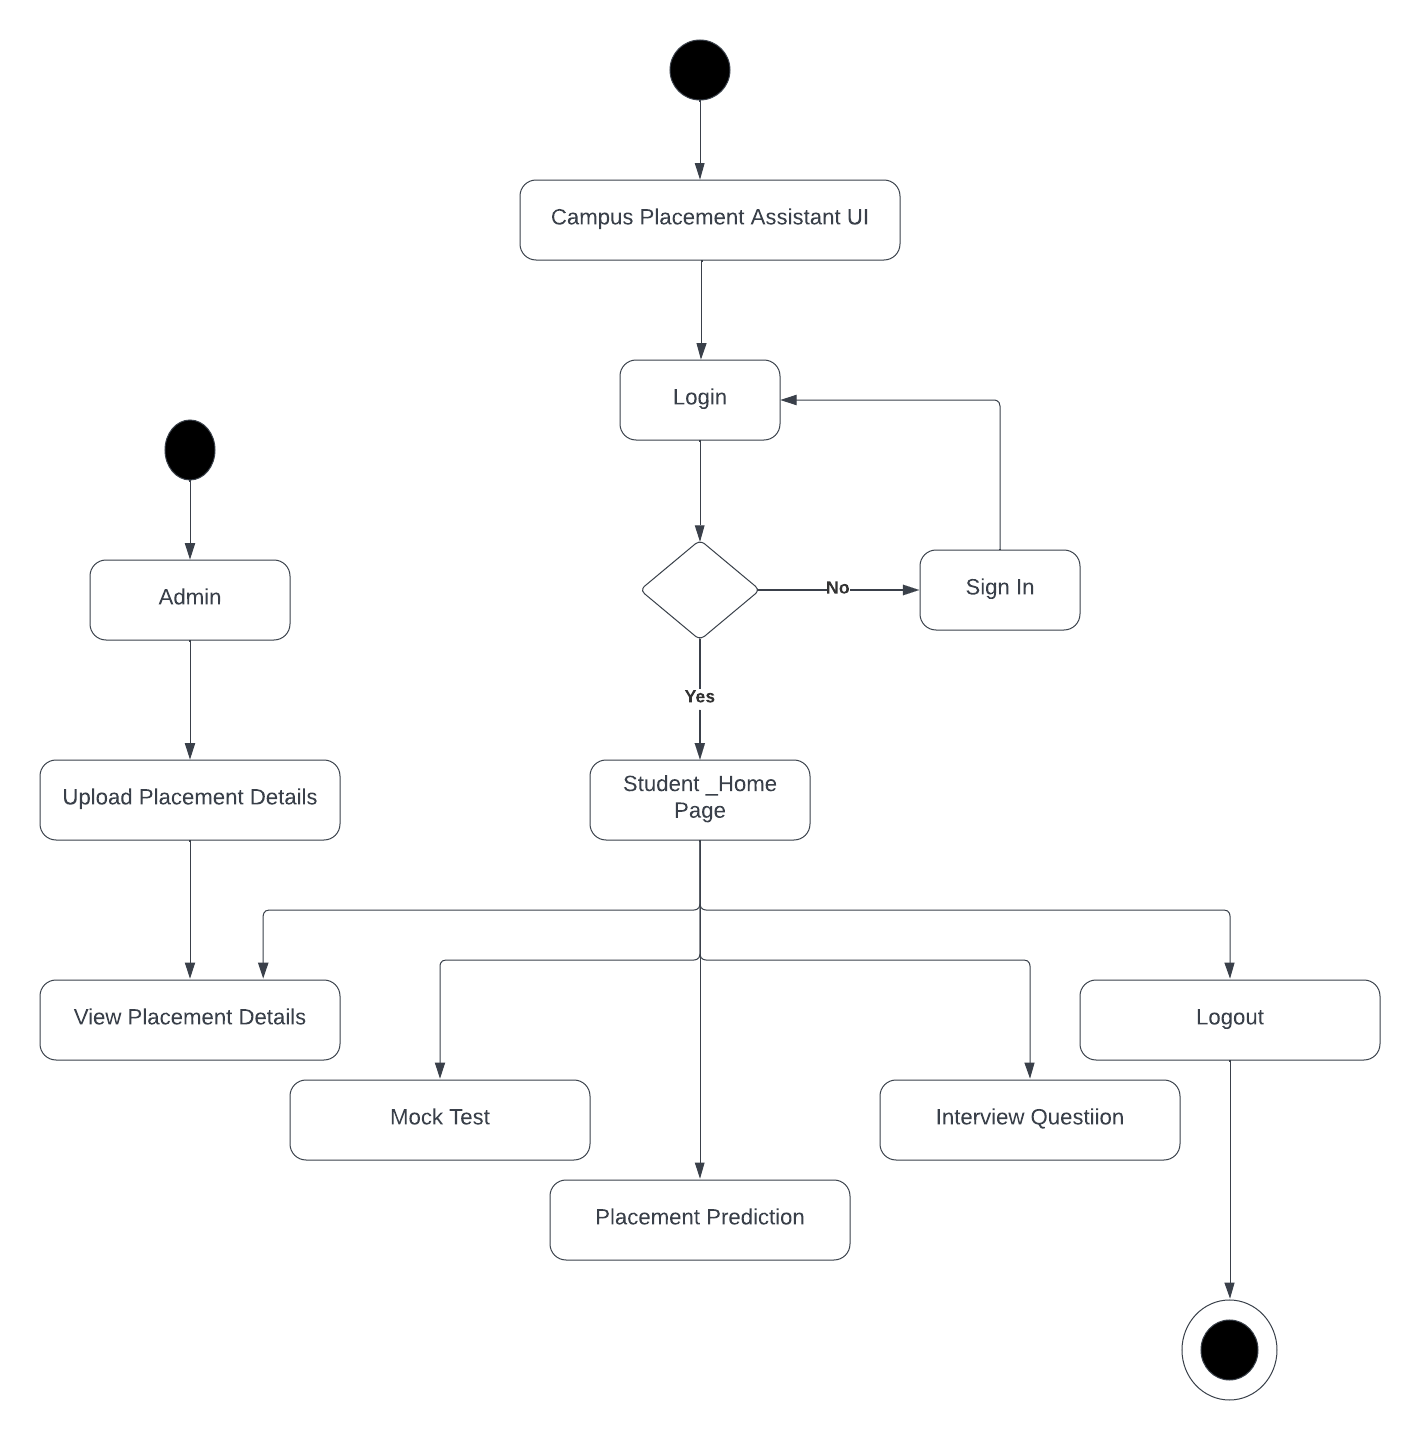
\includegraphics[scale=.8]{Activity diagram}
\caption{Activity Diagram}
\end{center}
\end{figure}
\newpage
\subsubsection{Class Diagram}

Class diagram is a static diagram. It represents the static view of an application. Class diagram is not only used for visualizing, describing, and documenting different aspects of a system but also for constructing executable code of the software application.

Class diagram describes the attributes and operations of a class and also the constraints imposed on the system. The class diagrams are widely used in the modeling of objectoriented systems because they are the only UML diagrams, which can be mapped directly with object-oriented languages.

Class diagram shows a collection of classes, interfaces, associations, collaborations, and constraints. It is also known as a structural diagram.

\begin{figure}[H]
\begin{center}
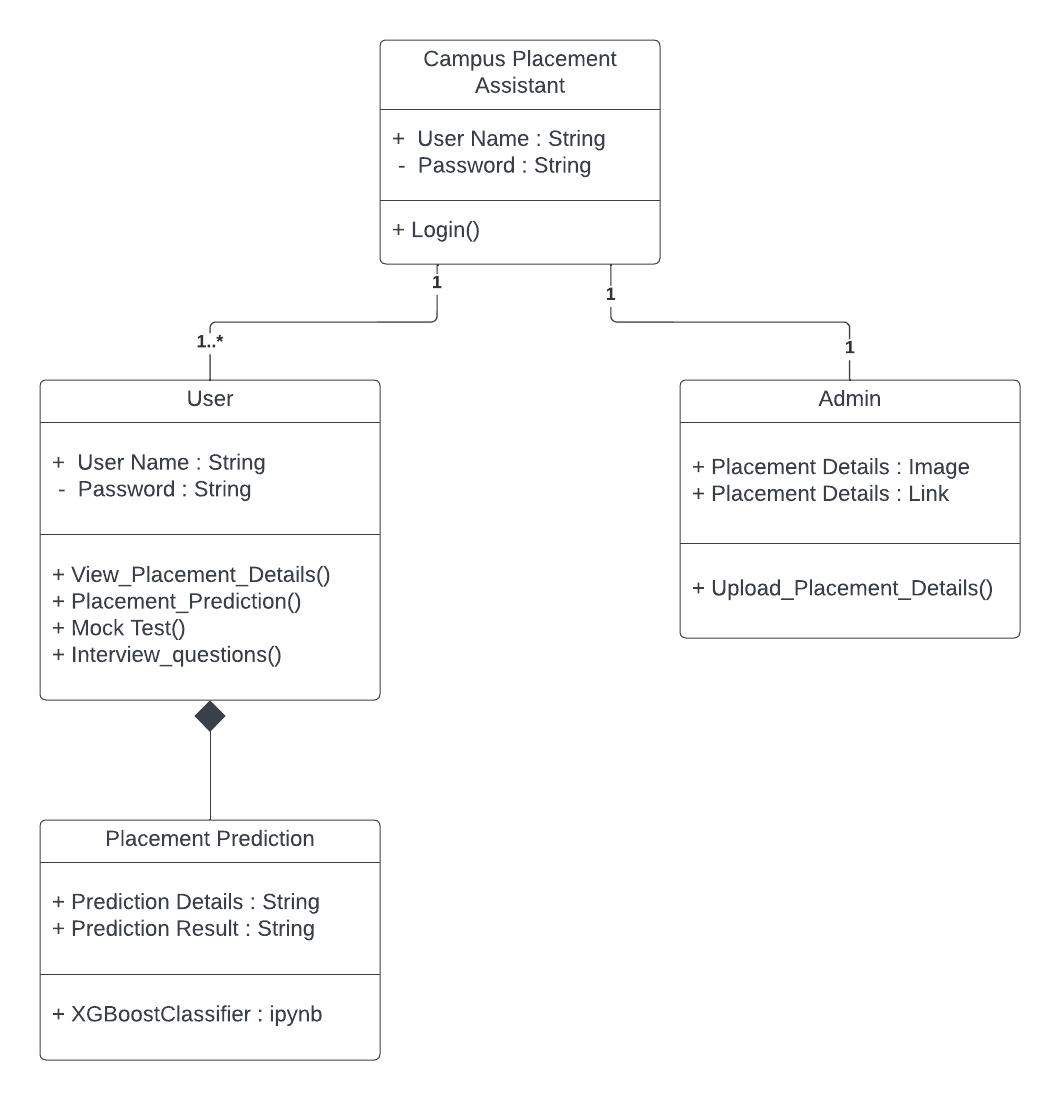
\includegraphics[scale=.6]{Class diagram}
\caption{Class Diagram}
\end{center}
\end{figure}

\newpage
\begin{flushleft}\textbf{CHAPTER 8} \end{flushleft}
\begin{flushleft}\section{IMPLEMENTATION} \end{flushleft}

\subsection{Module Description}

The system architecture depicts the overall working of our system .
\begin{figure}[H]
\begin{center}
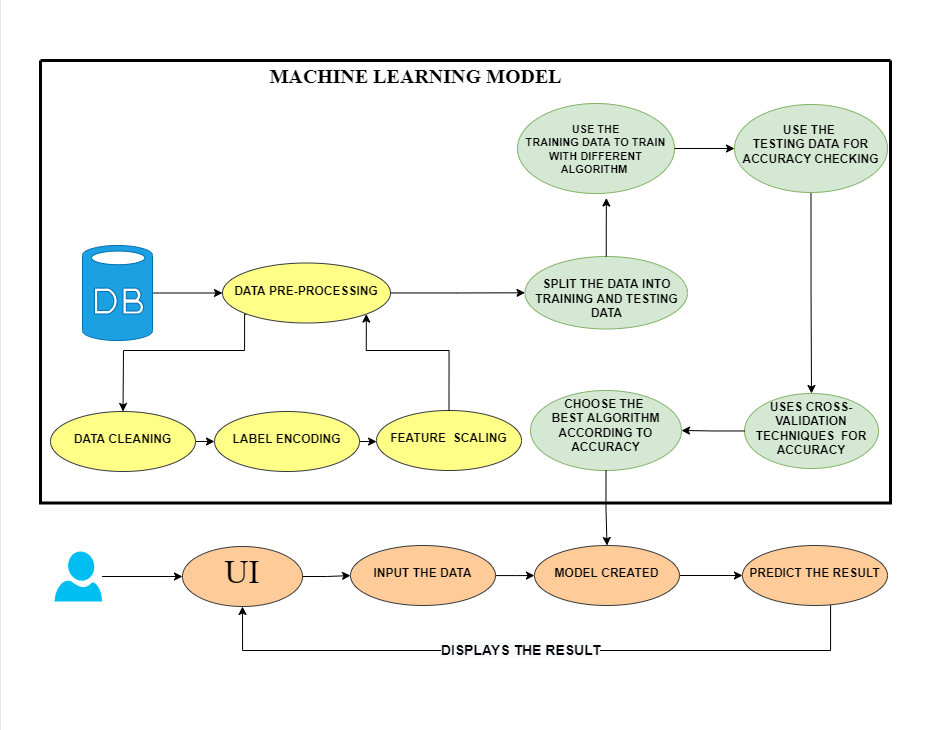
\includegraphics[scale=.7]{ML1}
\caption{System Architecture}
\end{center}
\end{figure}

The modules in the system architecture are:
\begin{itemize}

\item \textbf{Database:} The database contains the dataset of the student placement information from the previous year data. This data is used to train the machine learning model. 

\item \textbf{Data Pre-Processing:} 
Today's real world databases are highly susceptable to noisy, missing and inconsistent data due to their huge size and their lightly origin from multiple heterogeneous sources. Low quality data will lead to low quality Prediction results. Data prerocessing helps to improve the quality of the data and consequently of the Prediction results. Data preprocessing is a data mining technique which is used to transform the raw data in a useful and efficient format. There are several pre-processing techiniques such as :
\begin{enumerate}
\item \textbf{Data Cleaning:} It can be applied to remove noise and correct inconsistency in the data. It cleans the data by filling the missing values, smoothing noisy data, identify or removing outlayers and removing inconsistencies.
\item \textbf{Label Encoding:}
Label Encoding refers to converting the labels into a numeric form so as to convert them into the machine-readable form. Machine learning algorithms can then decide in a better way how those labels must be operated. It is an important pre-processing step for the structured dataset in supervised learning.
\item \textbf{Feature Scaling:}Feature Scaling or Standardization: It is a step of Data Pre Processing that is applied to independent variables or features of data. It basically helps to normalize the data within a particular range. Sometimes, it also helps in speeding up the calculations in an algorithm.
\end{enumerate}
\item \textbf{Splitting the Data:}
It splits the data into training and testing data where it uses the training data to train the machine learning algorithms with 80\% of the data and remianing 20\% data for testing the accuracy of the machine learning algorithm.
\item \textbf{Training:}
The training data is trained with the different machine learning algorithm such as Logistic regression, KNN Algorithm, SVM Algorithm, Decision Tree and XGBoost Classifier.
\item \textbf{Testing:} All the trained machine learning algorithms are being tested with testing data and accuracy of all the machine learning algorithms are compared to get the best machine learning algorithm.
\item \textbf{Prediction:} The best machine learning algorithm is used to predict the result of the individual prediction of the input taken from the user interface.
\end{itemize}
\subsection{Working}
The working of the system is described as follows :
\begin{steps}
  \item \textbf{Login:} Login to the campus placement assistant website by signing up with email or using google for sign up. After sign up with google or email it will show the respective email id used for sign up and the user can sign in to the Login using the password or google with security enabled.
  \item \textbf{Home Page:} The Login directs to the home page where I can go to options such as Placement Details, Placement Prediction, Mock Test and Interview Question.
\item \textbf{Placement Details:} The placement details shows the current placement updates that are uploaded by the admin. Students can view all those details and can apply for those jobs and this allows a dedicated environment for the students to go for placement details updated by the admin.
\item \textbf{Placement Prediction:}The student can check the probablity that they can get placed using placement predictor. The user details are transfered to deepnote after pressing the predict button, where the user details are used to predict the result by XGBoost classifier and the result is passed back to the placemnt prediction module as the person can get placed or not. If the person can't get placed the corresponding course details are displayed.
\item \textbf{Mock Test and Interview Question:} To get better placement student can go through these moudules where they can practice with mock test and familiarize with interview questions.
\item \textbf{Logout:} The user can logout and the page will be redirected to the sigin page.
\end{steps}

\newpage
\begin{flushleft}\textbf{CHAPTER 9} \end{flushleft}
\begin{flushleft}\section{TESTING} \end{flushleft}
\vspace*{10px}
This section describes the testing procedure, staring with the testing methodology
and then continuing with the tests performed on the system.
\begin{itemize}
\item Testing is a process of exceeding with the internet of finding an error.
\item A good test case is one that has a high probability of finding an undiscovered error.
\item A successful test is one that uncovers undiscovered errors.
\end{itemize}

\subsection{Testing Methodology}
The most natural and customary way of verifying any piece of work is just to operate
it in some representative situation and verify whether its behavior is as expected. In
general it is impossible to test it under all possible operating conditions. Thus it
is necessary to find suitable test cases that provide enough evidence that the desired
behavior will be exhibited in all remaining case. Testing is a critical activity in software
engineering and should be performed as systematically as possible by stating clearly
what result one expects from it and how one obtains these results. On the contrary,
often in practice, testing is performed in an unstructured way without applying any
criterion. There are two approaches to testing:
\begin{itemize}
\item White box testing

This is testing software using information about the internal structure of the software. It tests what the program does. The test is being carried out to check the internal structure of the software. The test is carried out successfully and the internal structure
of the software meets the required criteria.
\item Black box testing\\
Testing a piece of software as a black box (also called functional testing) means
operating the software without relying on any knowledge of the way it has been designed
and coded. It tests what it is supposed to do. The Programs run successfully against
task assigned.
\item  Unit Testing\\
This is the first level of testing. In this different modules are tested against the
specification produces during the design of the modules. Unit testing is done during
the coding phase and to test the internal logic of the modules. It refers to the modules.
It refers to the verification of single program module in an isolated environment.
Unit testing first focuses on the modules independently of one of another to locate errors.
After coding each dialogue is tested and run individually. All necessary coding were
removed and it was ensured that all modules are worked, as the programmer would
expect. The logical errors found were corrected so, by working all the modules independently and verifying the outputs of each module in the presence of staff, I observed
that the program was functioning as expected. In unit testing – Module is tested to
ensure that information properly flows into and out of the program under test – Local
data structures are examined to ensure that data stored temporarily maintains its integrity during all steps in algorithm execution. Boundary condition is tested to ensure
that module operates properly at boundaries established to limit or restrict processing.
– All independent paths through the control structures are executed to ensure that
all statements in the module have been executed at least once.
– Error handling paths are also tested.
\item Integration testing\\
Data can be lost across an interface: one module can be adversely affected on
another; sub functions when combine may not produce the desired major functions.
Integration testing is a systematic testing for constructing the program structure. Conducting the tests is to uncover errors associated within the interface. The objective
is to take unit tested to modules and build a program structure. All the modules are
combined and tested as a whole. Here correction is difficult because the vast expenses
of the entire program complicate the isolation of causes. Thus in the integration testing
step, all the errors uncovered are corrected for the next testing steps.\\
– Low – Level modules are combined to form clusters .\\
– The cluster is tested.\\
– Drivers are removed and clusters are combined moving upward in the program
structure.
\item  Alpha Testing\\
A series of acceptance tests were conducted to enable the users to validate requirements. The suggestions, along with the additional requirements of the end user were
included in the project.
\item Beta Testing\\
It is to be conducted by the end – user without the presence of the developer. It
can be conducted over a period of weeks or month. Since it is a long time consuming
activity, its result is out scope of this project report. But its result will help to enhance the product at a later time.
\item  Validation Testing\\
This provides final assurance that the software meets all the functional, behavioral
and performance requirement. The software is completely assembled as a package.
Validation succeeds when the software functions in a manner in which user wishes.
Validation refers to the process of using software in live environment in order to find
errors. During the course of validation the system failure may occur and sometimes
the coding has to be hanged according to the requirement. Thus the feedback from
the validation phase generally produces changes in software. Once the application was
made of all logical and interface errors, inputting dummy data ensure that the software
developed satisfied all the requirements of the user. This dummy data is known as test
case.
\item Output Testing\\
After performing the validation testing, the next step is output testing of the proposed system since no system could be useful if it does not produce the required output
in a specific format. Asking the users about the format required by them, tests the
output generated are considered into two ways. One is on screen and another is printed
format. The output format on the screen found to be correct as the format was designed
in the system design phase according to the user needs. For the hard copy also, the
output comes out as the specified requirement by the user. Hence output testing does
not result in any correction in the system.
\end{itemize}

\newpage
\begin{flushleft}\textbf{CHAPTER 10} \end{flushleft}
\begin{flushleft}\section{RESULT} \end{flushleft}
The placement predictor predicts that a student can be placed or not .
\textbf{Placed}
\begin{figure}[H]
\begin{center}
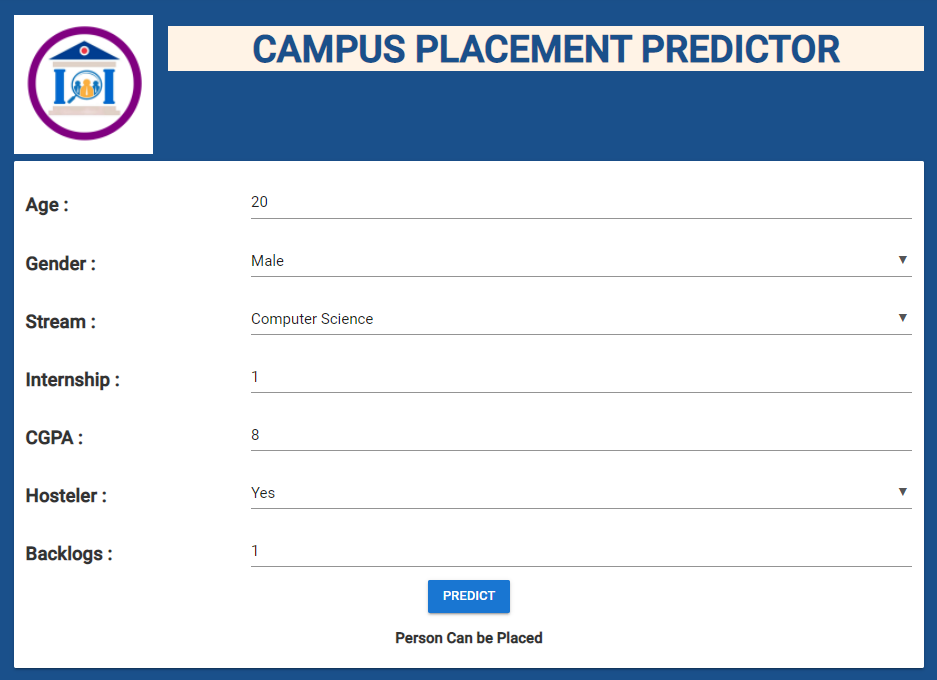
\includegraphics[scale=.4]{Result}
\caption{Student Predicted to be Placed}
\end{center}
\end{figure}
\textbf{Not Placed}
\begin{figure}[H]
\begin{center}
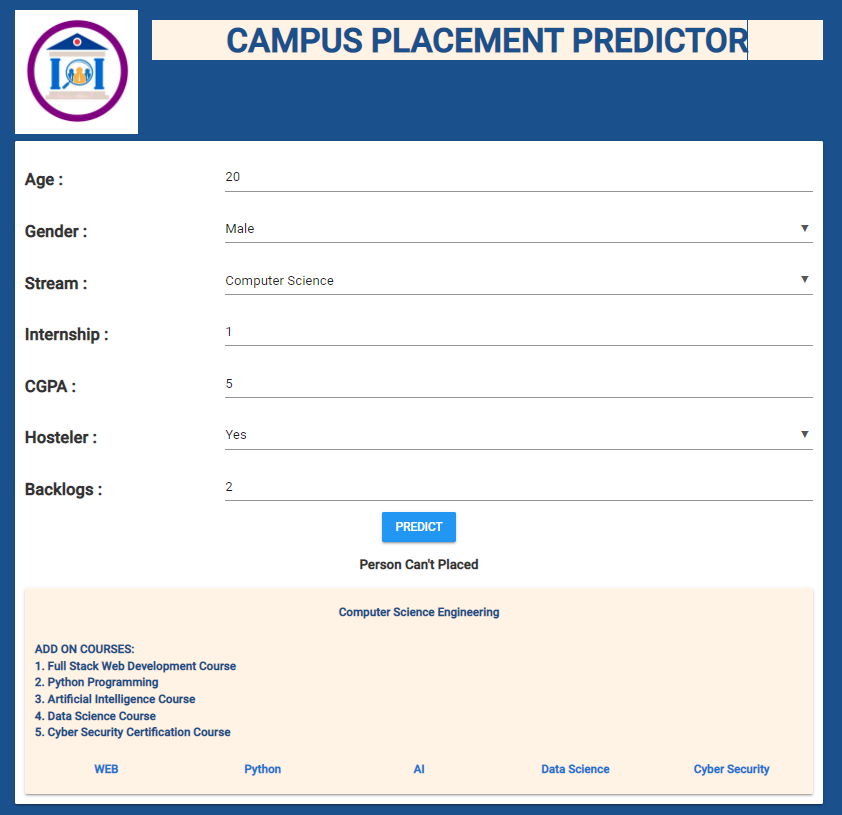
\includegraphics[scale=.4]{Result0}
\caption{Student Predicted to be not Placed}
\end{center}
\end{figure}
\begin{flushleft}\textbf{CHAPTER 11} \end{flushleft}
\begin{flushleft}\section{PERFOMANCE AND EVALUATION} \end{flushleft}
The campus placement assistant uses the placement predictor to predict whether a student can be placd or not and for prediction I have derived to  XGBoost Classifier and to check the accuracy of the model confusion matrix has been used, the confusion matrix conveys the visual representation of the Actual VS Predicted values. It measures the performance of our Machine Learning classification model and looks like a table-like structure.
\begin{figure}[H]
\begin{center}
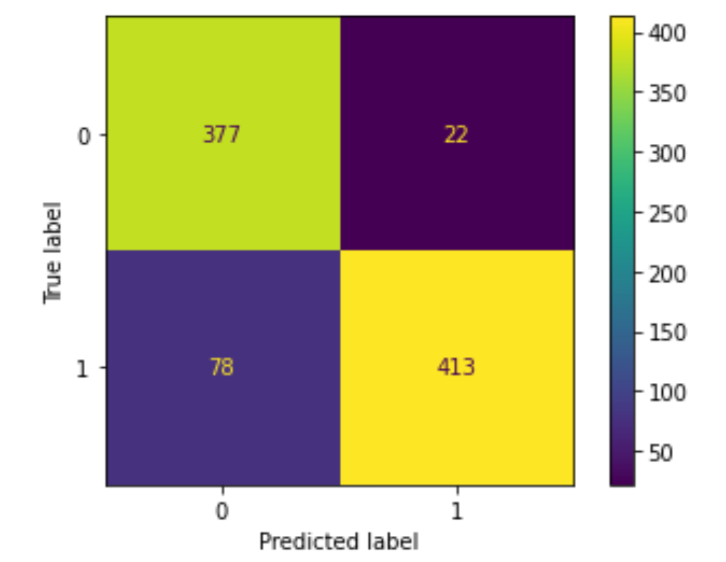
\includegraphics[scale=.4]{ResultP1}
\caption{Confusion Matrix for XGBoost classifier}
\end{center}
\end{figure}
The different values of the Confusion matrix would be as follows:
\begin{itemize}
\item \textbf{True Positive:} (TP) = 377; meaning 377 positive class data points were correctly classified by the model
\item \textbf{True Negative:} (TN) = 413; meaning 413 negative class data points were correctly classified by the model
\item \textbf{False Positive:} (FP) = 22; meaning 22 negative class data points were incorrectly classified as belonging to the positive class by the model
\item \textbf{False Negative:} (FN) = 78; meaning 78 positive class data points were incorrectly classified as belonging to the negative class by the model
\end {itemize}
The graphs such as Area Under Curve AUC and Average Precision AP has been found :
\textbf{AUC:}
The AUC indicates whether your model can correctly rank examples. The AUC is the probability that a randomly selected positive example has a higher predicted probability of being positive than a randomly selected negative example. The AUC is calculated as the area underneath a curve that measures the trade off between true positive rate (TPR) and false positive rate (FPR) at different decision thresholds d.
\begin{figure}[H]
\begin{center}
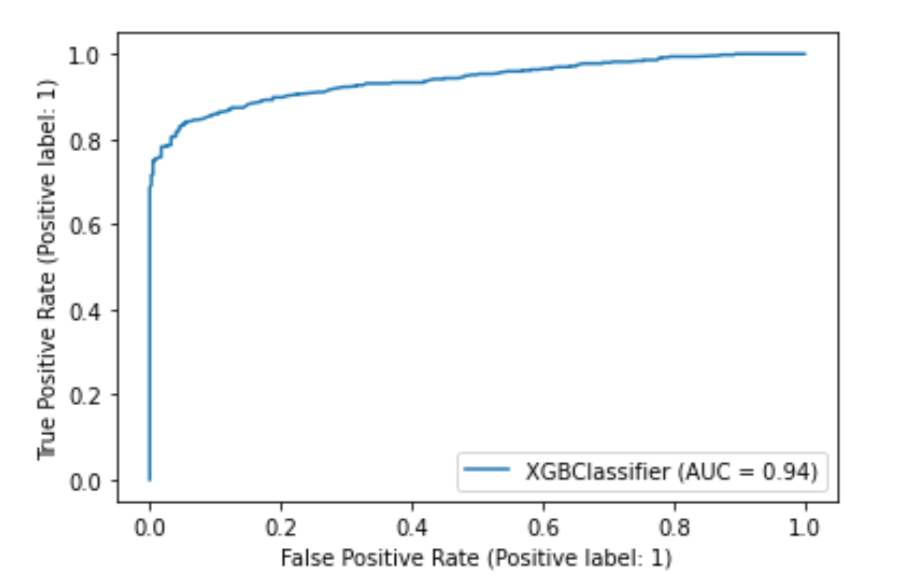
\includegraphics[scale=.4]{ResultP2}
\caption{AUC for XGBoost classifier}
\end{center}
\end{figure}
\textbf{AP:}
Average precision indicates whether your model can correctly identify all the positive examples without accidentally marking too many negative examples as positive. Thus, average precision is high when your model can correctly handle positives. Average precision is calculated as the area under a curve that measures the trade off between precision and recall at different decision thresholds.
\begin{figure}[H]
\begin{center}
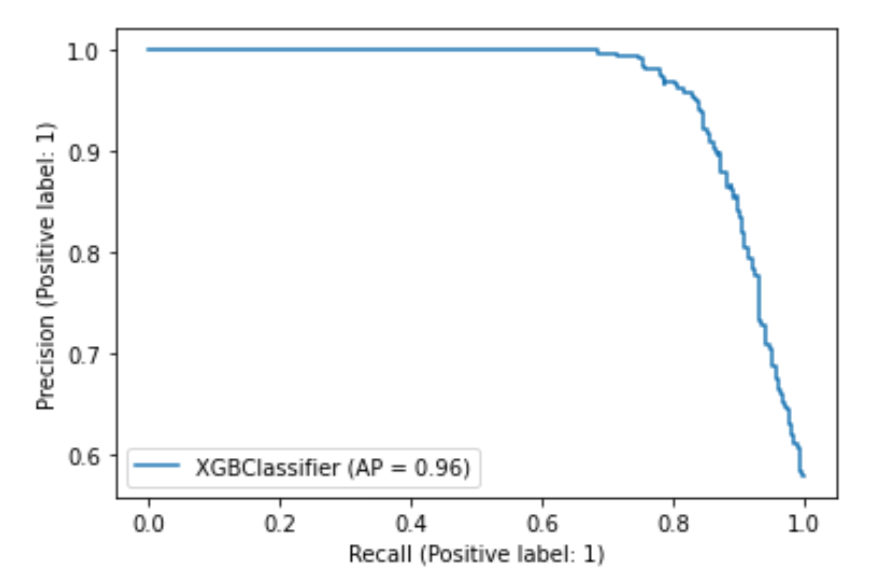
\includegraphics[scale=.4]{ResultP3}
\caption{AP for XGBoost classifier}
\end{center}
\end{figure}
The result that I obtained using XGBoost classifier has got about 89\% of accuracy.
\newpage
\begin{flushleft}\textbf{CHAPTER 12} \end{flushleft}
\begin{flushleft}\section{SCREENSHOT} \end{flushleft}

\begin{figure}[H]
\begin{center}
 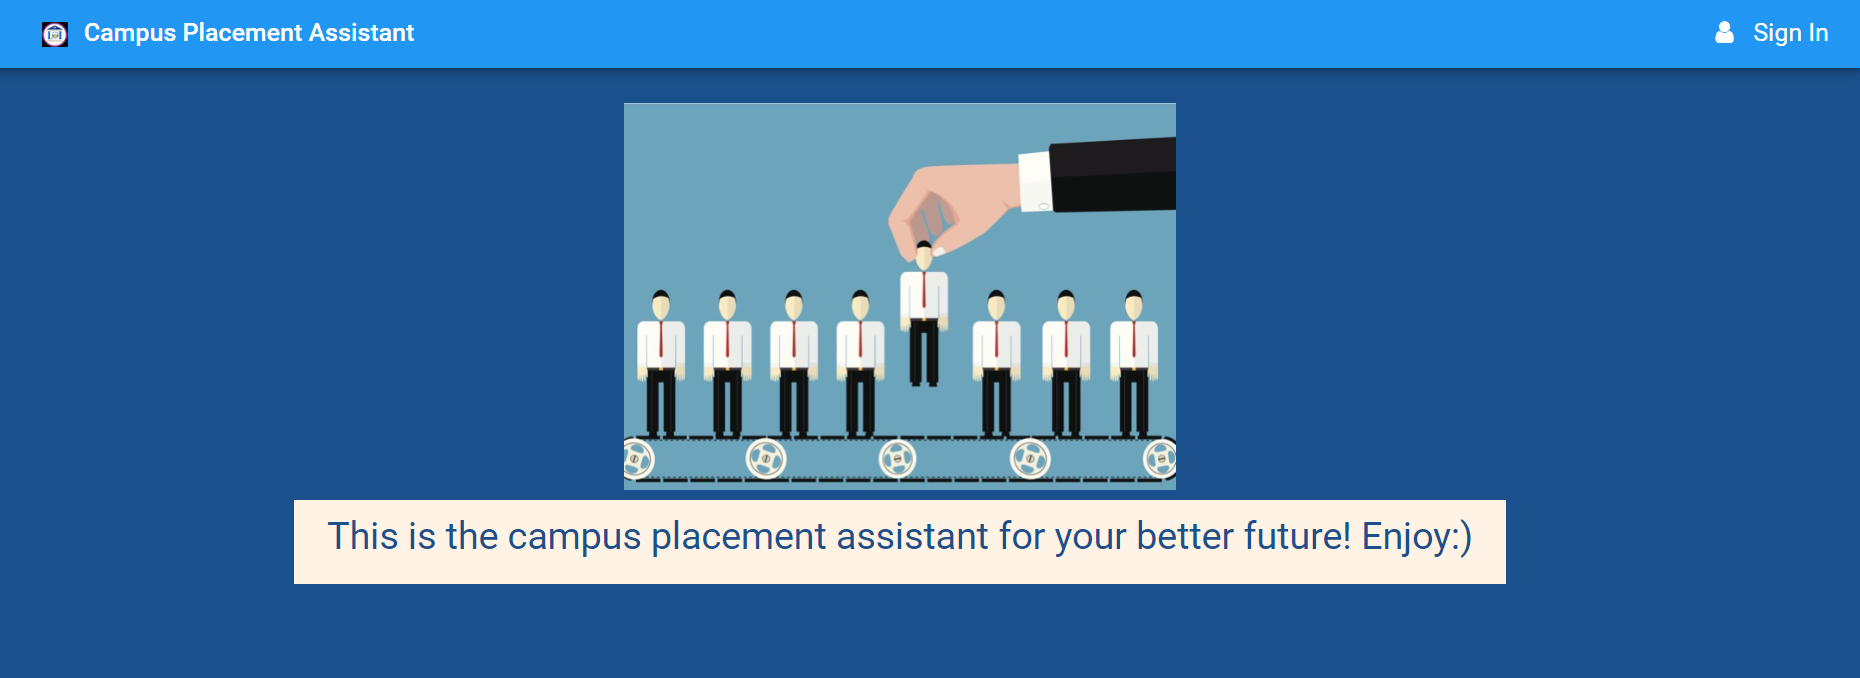
\includegraphics[width=16cm, height=8cm]{Screenshot1}
\caption{Login Page }
\end{center}
\end{figure}

\begin{figure}[H]
\begin{center}
 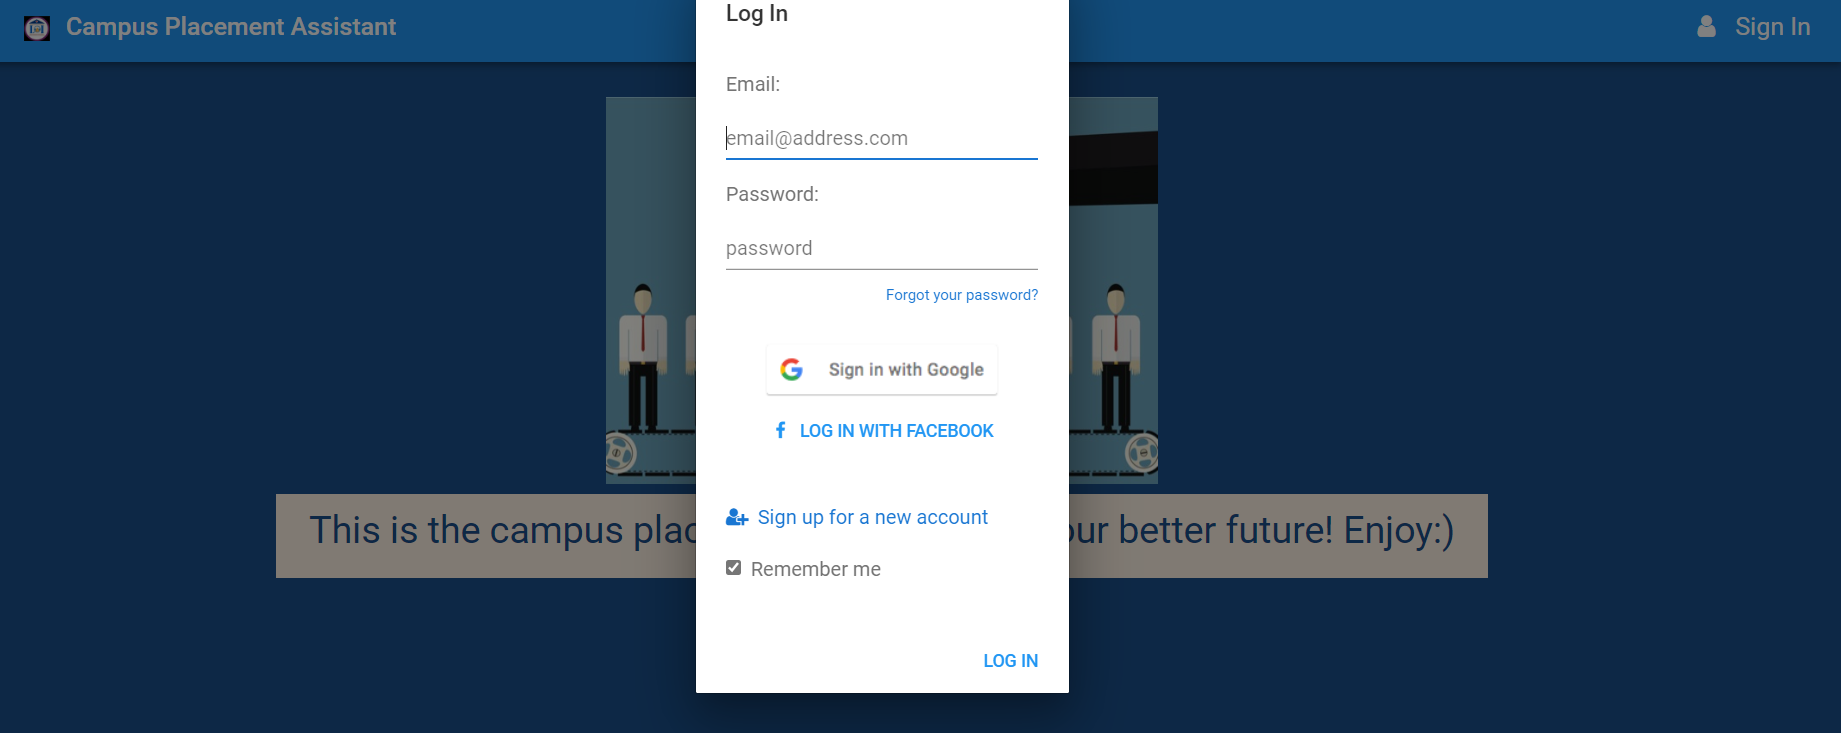
\includegraphics[width=16cm, height=8cm]{Screenshot2}
\caption{Sign Up Page}
\end{center}
\end{figure}

\begin{figure}[H]
\begin{center}
 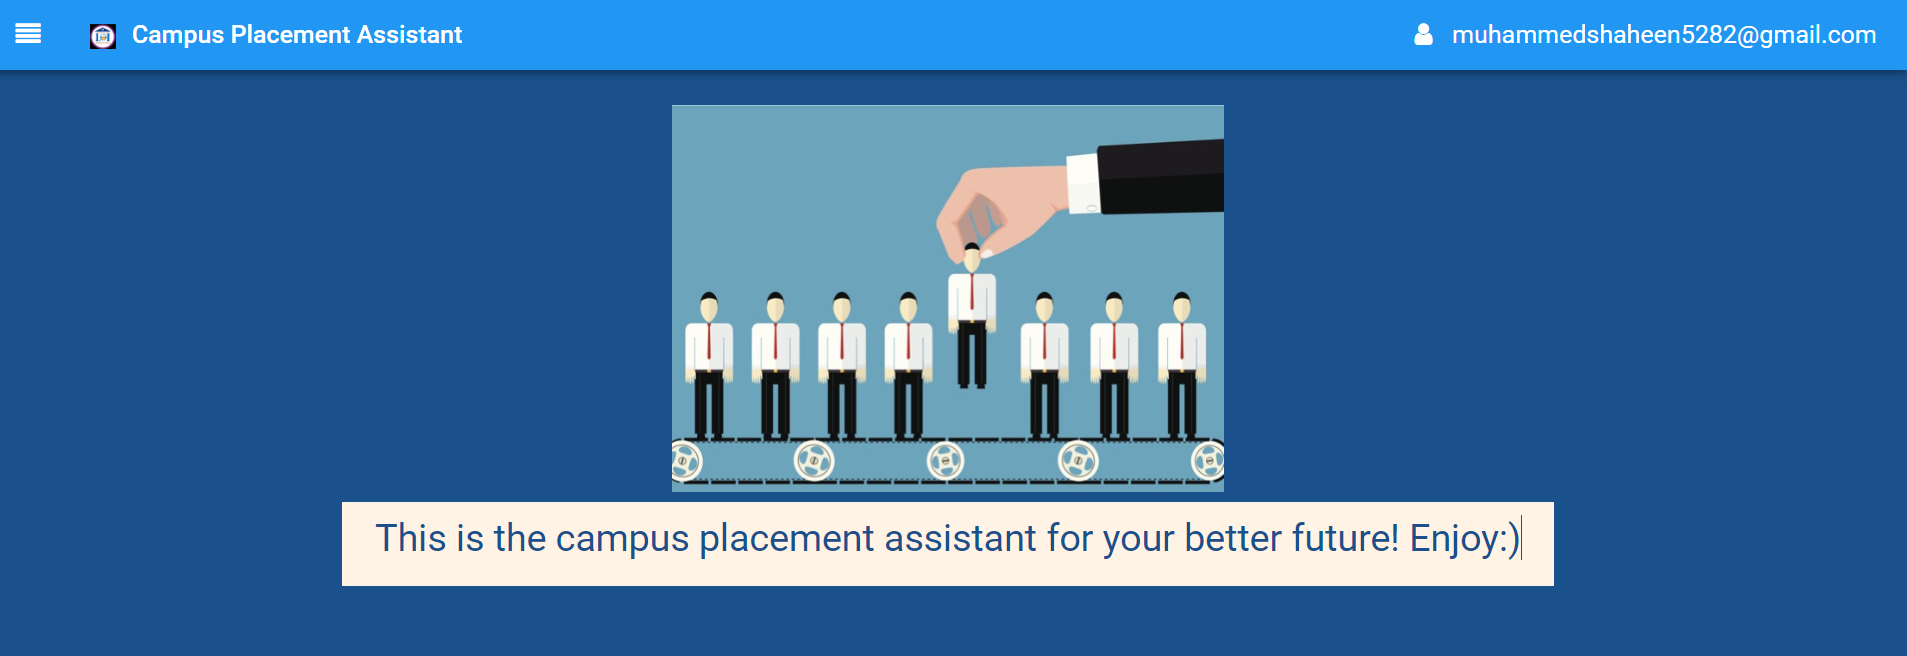
\includegraphics[width=16cm, height=8cm]{Screenshot3}
\caption{Home Page }
\end{center}
\end{figure}

\begin{figure}[H]
\begin{center}
 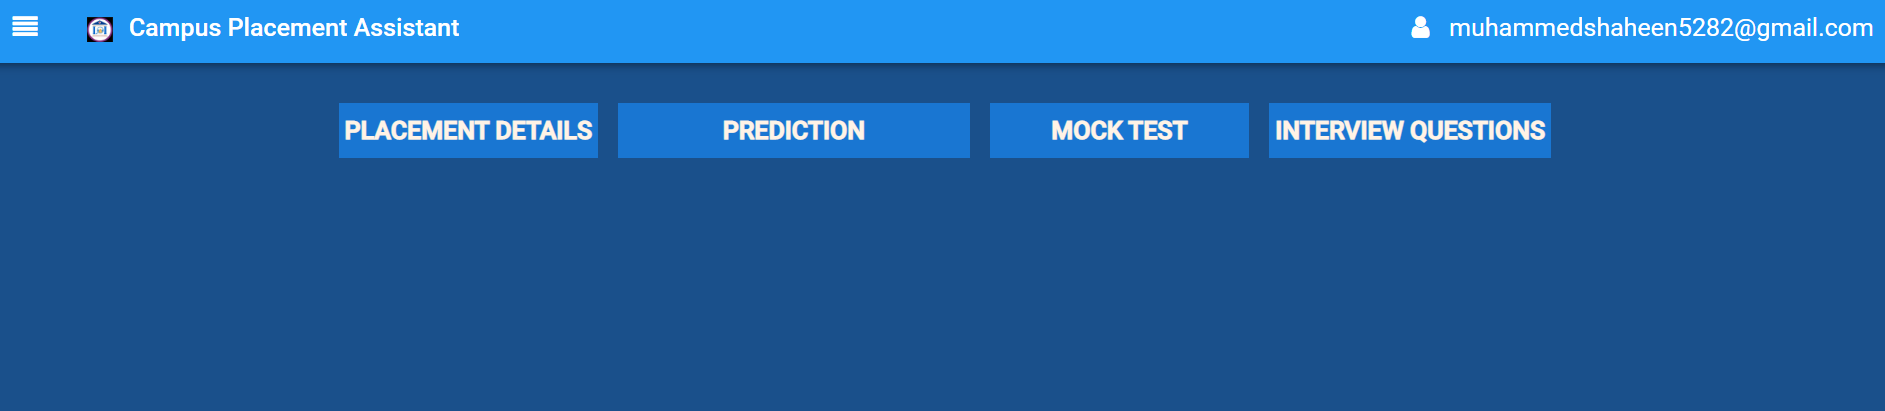
\includegraphics[width=16cm, height=8cm]{Screenshot4}
\caption{Other options}
\end{center}
\end{figure}

\begin{figure}[H]
\begin{center}
 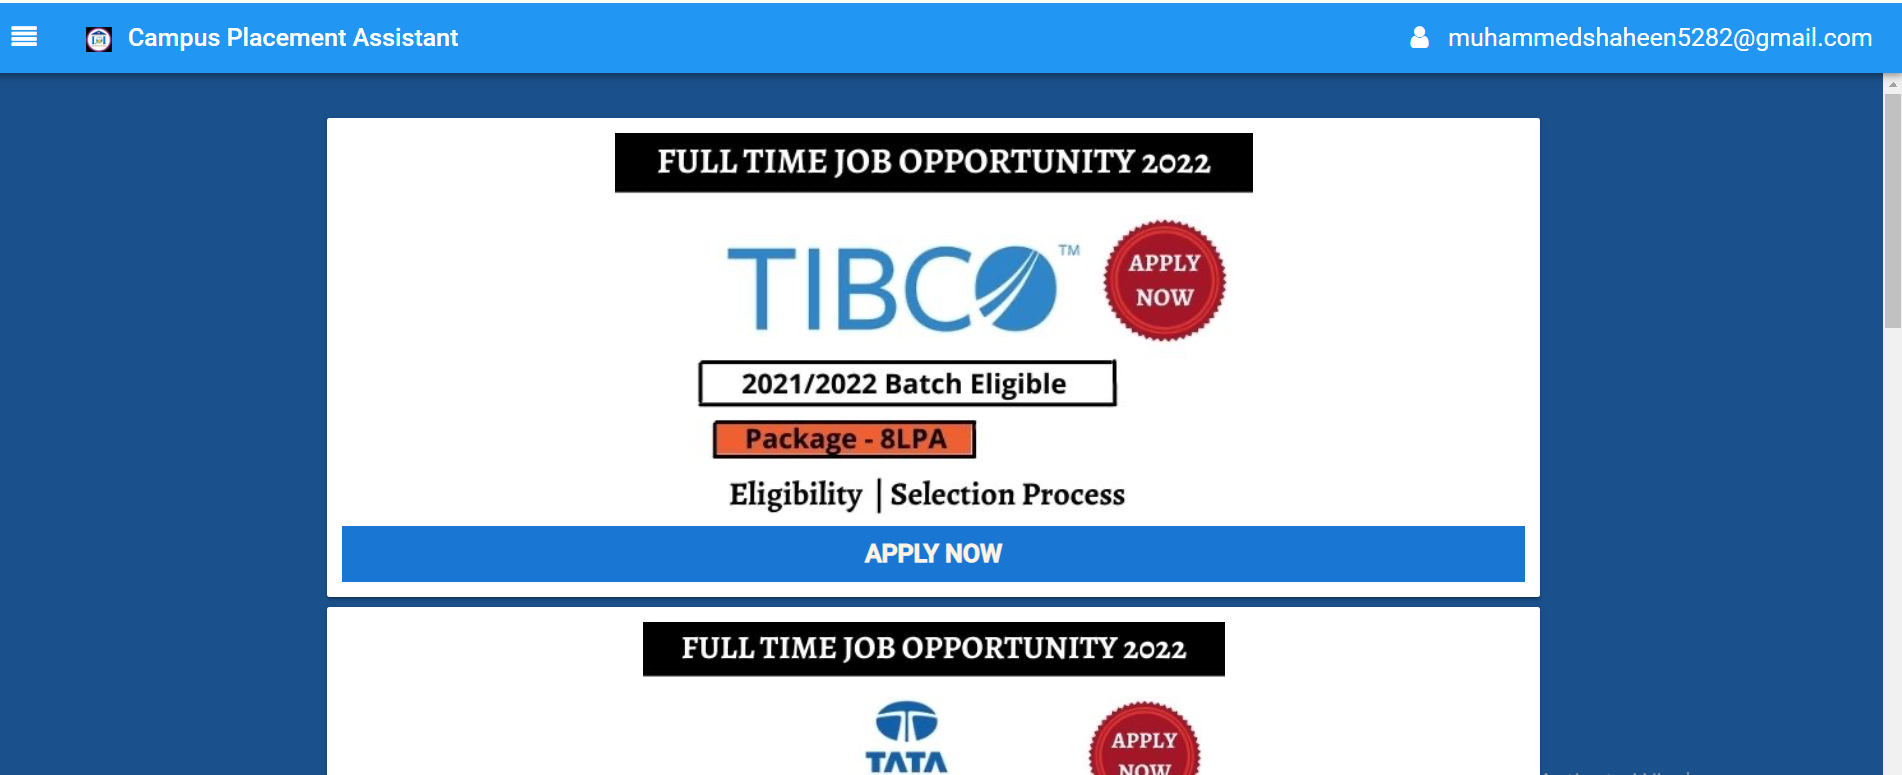
\includegraphics[width=16cm, height=8cm]{Screenshot5}
\caption{Placement Details}
\end{center}
\end{figure}

\begin{figure}[H]
\begin{center}
 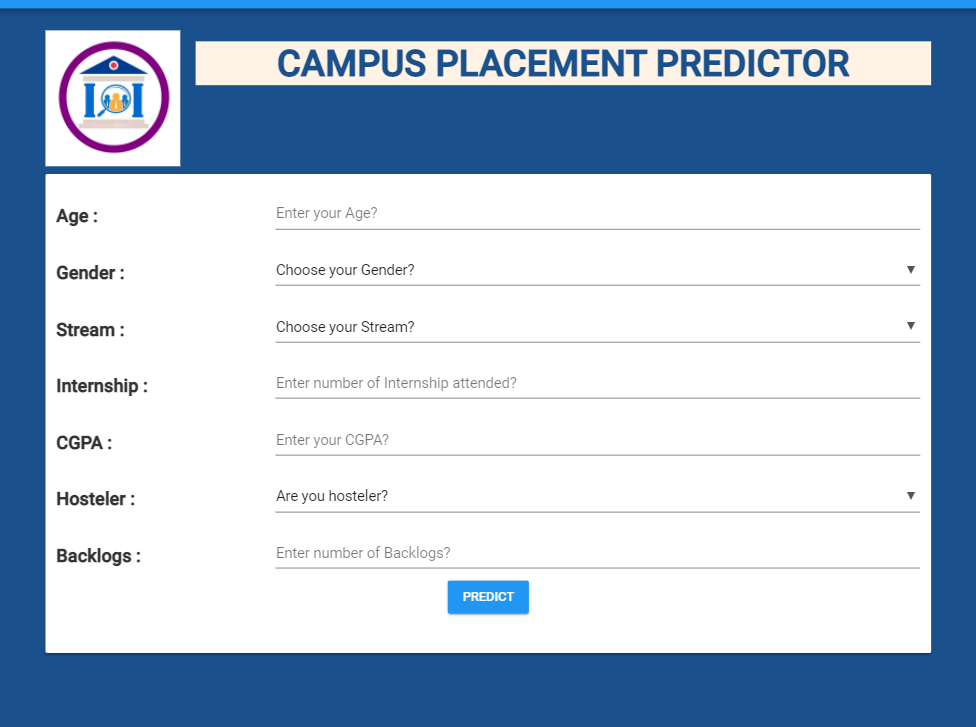
\includegraphics[width=16cm, height=8cm]{Screenshot6}
\caption{Placement Prediction}
\end{center}
\end{figure}

\newpage


\begin{flushleft}\textbf{CHAPTER 13} \end{flushleft}
\begin{flushleft}\section{CONCLUSION} \end{flushleft}
The campus placement assistant will hep the student to get all the placement support in a nutshell that include placement details from the admin, placement prediction using the best machine learning algorithm, mock test and interview question. In the case of Placement Prediction a point-by - point analysis was performed based on specific 
machine learning algorithms for predicting the placement probablity and XGBoost classifier has the best accuracy with 89\%. The student dataset including academic and selection subtleties is clearly a 
possible hotspot from the exam for forecasting future selection 
possibilities. Such forecast will empower students to consider 
their skills and develop according to their needs. This 
methodology also helps to prepare appropriate procedures and 
strengthen the recruitment statistics for future years in the 
scholastic arrangement of an establishment. The placement officer of a campus can also benefit from this system to have an organised platform for placement.



\newpage
\renewcommand{\thepage}{}
\begin{center}

\end{center}
\addcontentsline{toc}{section}{REFERENCES}
     \begin{thebibliography}{99}
\bibitem{title}
 Performance Comparison of Machine Learning Algorithms for Prediction ofg Students’ 
Social Engagement https://doi.org/10.1109/ICCMC51019.2021.9418260

\bibitem{second}
An EDM Approach to the Analysis of Students' Engagement in Online Courses from 
Constructs of the Transactional Distance https://doi.org/10.1109/ICALT.2016.17

\bibitem{third}
Using Ranking and Multiple Linear Regression to Explore the Impact of Social Media 
Engagement on Student Performance https://doi.org/10.1109/ICALT.2016.140

\bibitem{fourth}
Student Academic Performance and Social Behavior Predictor using Data Mining Techniques 
https://doi.org/10.1109/CCAA.2017.8229794

\bibitem{fifth}
 Student Engagement Predictions in an e-Learning System and Their Impact on Student 
Course Assessment Scores https://doi.org/10.1155/2018/6347186
\bibitem{sixth}
 Cluster and Logistic Regression Distribution of Students’ Performance by Classification 


\end{thebibliography} gr

\end{document}





































